
\documentclass[12pt, a4paper]{article}

% -----------------------------------------------------------
% КОДИРОВКА И ЯЗЫК (XeLaTeX)
% -----------------------------------------------------------
\usepackage{fontspec}
\usepackage{polyglossia}
\setmainlanguage{russian}
\setotherlanguage{english}
\setmainfont{FreeSerif}
\setmonofont{FreeMono}

% -----------------------------------------------------------
% МАТЕМАТИКА
% -----------------------------------------------------------
\usepackage{amsmath, amssymb, amsthm}
\usepackage{mathtools}
\usepackage{float} % BẮT BUỘC để dùng [H]
% -----------------------------------------------------------
% ГРАФИКА
% -----------------------------------------------------------
\usepackage{graphicx}
\usepackage{float}
\usepackage{subcaption}

% -----------------------------------------------------------
% ТАБЛИЦЫ
% -----------------------------------------------------------
\usepackage{booktabs}
\usepackage{multirow}
\usepackage{array}

% -----------------------------------------------------------
% ЛИСТИНГИ КОДА
% -----------------------------------------------------------
\usepackage{listings}
\usepackage{xcolor}

\definecolor{codebg}{RGB}{245,245,245}
\definecolor{codeframe}{RGB}{200,200,200}
\definecolor{kw}{RGB}{0,0,160}
\definecolor{cm}{RGB}{60,120,60}
\definecolor{st}{RGB}{160,0,0}

\lstset{
    language=Python,
    basicstyle=\ttfamily\footnotesize,
    backgroundcolor=\color{codebg},
    frame=single,
    rulecolor=\color{codeframe},
    keywordstyle=\color{kw}\bfseries,
    commentstyle=\color{cm}\itshape,
    stringstyle=\color{st},
    breaklines=true,
    breakatwhitespace=true,
    keepspaces=true,       
    columns=fullflexible,  
    showstringspaces=false,
    numbers=left,
    numberstyle=\tiny\color{gray},
    numbersep=8pt,
    tabsize=4,
    captionpos=b,
    extendedchars=true,
    inputencoding=utf8,
    literate=
      {а}{{\selectlanguage{russian}а}}1
      {б}{{\selectlanguage{russian}б}}1
      {в}{{\selectlanguage{russian}в}}1
      {г}{{\selectlanguage{russian}г}}1
      {д}{{\selectlanguage{russian}д}}1
      {е}{{\selectlanguage{russian}е}}1
      {ж}{{\selectlanguage{russian}ж}}1
      {з}{{\selectlanguage{russian}з}}1
      {и}{{\selectlanguage{russian}и}}1
      {й}{{\selectlanguage{russian}й}}1
      {к}{{\selectlanguage{russian}к}}1
      {л}{{\selectlanguage{russian}л}}1
      {м}{{\selectlanguage{russian}м}}1
      {н}{{\selectlanguage{russian}н}}1
      {о}{{\selectlanguage{russian}о}}1
      {п}{{\selectlanguage{russian}п}}1
      {р}{{\selectlanguage{russian}р}}1
      {с}{{\selectlanguage{russian}с}}1
      {т}{{\selectlanguage{russian}т}}1
      {у}{{\selectlanguage{russian}у}}1
      {ф}{{\selectlanguage{russian}ф}}1
      {х}{{\selectlanguage{russian}х}}1
      {ц}{{\selectlanguage{russian}ц}}1
      {ч}{{\selectlanguage{russian}ч}}1
      {ш}{{\selectlanguage{russian}ш}}1
      {щ}{{\selectlanguage{russian}щ}}1
      {ъ}{{\selectlanguage{russian}ъ}}1
      {ы}{{\selectlanguage{russian}ы}}1
      {ь}{{\selectlanguage{russian}ь}}1
      {э}{{\selectlanguage{russian}э}}1
      {ю}{{\selectlanguage{russian}ю}}1
      {я}{{\selectlanguage{russian}я}}1
      {А}{{\selectlanguage{russian}А}}1
      {Б}{{\selectlanguage{russian}Б}}1
      {В}{{\selectlanguage{russian}В}}1
      {Г}{{\selectlanguage{russian}Г}}1
      {Д}{{\selectlanguage{russian}Д}}1
      {Е}{{\selectlanguage{russian}Е}}1
      {З}{{\selectlanguage{russian}З}}1
      {И}{{\selectlanguage{russian}И}}1
      {К}{{\selectlanguage{russian}К}}1
      {Л}{{\selectlanguage{russian}Л}}1
      {М}{{\selectlanguage{russian}М}}1
      {Н}{{\selectlanguage{russian}Н}}1
      {О}{{\selectlanguage{russian}О}}1
      {П}{{\selectlanguage{russian}П}}1
      {Р}{{\selectlanguage{russian}Р}}1
      {С}{{\selectlanguage{russian}С}}1
      {Т}{{\selectlanguage{russian}Т}}1
      {У}{{\selectlanguage{russian}У}}1
      {Ф}{{\selectlanguage{russian}Ф}}1
      {Х}{{\selectlanguage{russian}Х}}1
      {Ц}{{\selectlanguage{russian}Ц}}1
      {Ч}{{\selectlanguage{russian}Ч}}1
      {Ш}{{\selectlanguage{russian}Ш}}1
      {Щ}{{\selectlanguage{russian}Щ}}1
      {Э}{{\selectlanguage{russian}Э}}1
      {Ю}{{\selectlanguage{russian}Ю}}1
      {Я}{{\selectlanguage{russian}Я}}1
}

% -----------------------------------------------------------
% ПОЛЯ И ОФОРМЛЕНИЕ
% -----------------------------------------------------------
\usepackage{geometry}
\geometry{left=2.5cm, right=2cm, top=2.5cm, bottom=2.5cm}

\usepackage{hyperref}
\hypersetup{
    colorlinks=true,
    linkcolor=blue,
    urlcolor=blue,
    citecolor=blue
}

\usepackage{enumitem}
\usepackage{parskip}
\setlength{\parindent}{0pt}
\setlength{\parskip}{5pt}

\usepackage{fancyhdr}
\pagestyle{fancy}
\fancyhf{}
\rhead{\small Лабораторная работа №4}
\lhead{\small «Линейные системы автоматического управления»}
\cfoot{\thepage}
\renewcommand{\headrulewidth}{0.4pt}

% ===========================================================
\begin{document}
% ===========================================================

% -----------------------------------------------------------
% ТИТУЛЬНАЯ СТРАНИЦА
% -----------------------------------------------------------
\begin{titlepage}
\pagenumbering{gobble} 
    \begin{center}
        \textbf{МИНИСТЕРСТВО НАУКИ И ВЫСШЕГО ОБРАЗОВАНИЯ РОССИЙСКОЙ ФЕДЕРАЦИИ}
        \\
        \textbf{ФЕДЕРАЛЬНОЕ ГОСУДАРСТВЕННОЕ АВТОНОМНОЕ ОБРАЗОВАТЕЛЬНОЕ УЧРЕЖДЕНИЕ ВЫСШЕГО ОБРАЗОВАНИЯ}
        \\
        \textbf{«Национальный исследовательский университет ИТМО»}
        \\
        \vspace{0.5cm}
        \textbf{ФАКУЛЬТЕТ СИСТЕМ УПРАВЛЕНИЯ И РОБОТОТЕХНИКИ}
        \\
        \vspace{3cm}
        \textbf{\Large ОТЧЕТ ПО ЛАБОРАТОРНОЙ РАБОТЕ №4} \\
        \vspace{0.5cm}
        \textbf{\large по дисциплине «Линейные системы автоматического управления»} \\
        \vspace{2cm}
        \textbf{ по теме:}
        \\
        \vspace{0.5cm}
        \textbf{\Large Типовые динамические звенья}
       
    \end{center}
    
    \vspace{3cm}
    
    \begin{flushright}
        \textbf{Выполнили:} \\
        Басиони Абдельсалам Али Абдельсалам\\
        Боврджи Тамим Махер Мохаммед\\
        Май Хоанг Куан \\
        
        
        \vspace{0.5cm}
        \textbf{Преподаватель:} \\
        Пашенко Артем Витальевич



    \end{flushright}
    
    \vfill
    
    \begin{center}
        Санкт-Петербург \\
        2026
    \end{center}
\end{titlepage}
\pagenumbering{arabic}
\tableofcontents

\graphicspath{{images/}}
% -----------------------------------------------------------
\newpage
\section{Объект 1: Двигатель постоянного тока}

\subsection{Передаточная функция объекта в стандартизированном виде и значения параметров}

\textbf{Исходные данные (Вариант 3):}

Динамика двигателя постоянного тока независимого возбуждения (без учета индуктивности якорной обмотки) описывается следующей системой уравнений:
\begin{equation}
    J\dot{\omega} = M, \quad M = k_m I, \quad I = \frac{U + \varepsilon_i}{R}, \quad \varepsilon_i = -k_e\omega,
\end{equation}
где входом объекта является напряжение питания $U(t)$, а выходом — угловая скорость вращения ротора $\omega(t)$.

Значения физических параметров для варианта 3 приведены в таблице \ref{tab:obj1_params}.

\begin{table}[H]
\centering
\caption{Параметры Объекта 1 (Вариант 3)}
\label{tab:obj1_params}
\setlength{\tabcolsep}{10pt} % Tăng khoảng cách đệm giữa các cột
\renewcommand{\arraystretch}{1.3} % Tăng chiều cao của các dòng cho thoáng
\begin{tabular}{@{} >{\raggedright\arraybackslash}p{3cm} >{\raggedright\arraybackslash}p{8.5cm} c @{}}
\toprule
\textbf{Обозначение} & \textbf{Наименование параметра} & \textbf{Значение} \\ \midrule
$k_m$ & Конструктивная постоянная по моменту, $\text{Н}\cdot\text{м/А}$ & $0.3637$ \\
$k_e$ & Конструктивная постоянная по ЭДС, $\text{В}\cdot\text{с}$ & $0.3637$ \\
$J$   & Момент инерции ротора, $\text{кг}\cdot\text{м}^2$ & $0.0023$ \\
$R$   & Активное сопротивление обмоток ротора, $\text{Ом}$ & $4.6050$ \\ \bottomrule
\end{tabular}
\end{table}


Подставим выражения для ЭДС вращения $\varepsilon_i$, тока $I$ и электромагнитного момента $M$ в уравнение движения ротора:
\begin{equation}
    J\dot{\omega}(t) = k_m \frac{U(t) - k_e\omega(t)}{R} \implies \frac{JR}{k_m k_e}\dot{\omega}(t) + \omega(t) = \frac{1}{k_e}U(t)
\end{equation}

Применив прямое преобразование Лапласа при нулевых начальных условиях ($\omega(0) = 0$), получим уравнение в операторной форме:
\[
    \left(\frac{JR}{k_m k_e}s + 1\right)\Omega(s) = \frac{1}{k_e}U(s).
\]
Отсюда передаточная функция объекта в стандартизированной форме имеет вид:
\begin{equation}
    W_1(s) = \frac{\Omega(s)}{U(s)} = \frac{K}{Ts + 1},
\end{equation}
где коэффициент усиления $K$ и постоянная времени $T$ определяются выражениями:
\[
    K = \frac{1}{k_e}, \quad T = \frac{JR}{k_m k_e}.
\]

\textbf{Расчет численных значений параметров $K$ и $T$:}
\[
    K = \frac{1}{0.3637} \approx 2.7495 \text{ (рад/с)/В}, \qquad T = \frac{0.0023 \cdot 4.6050}{0.3637 \cdot 0.3637} = \approx 0.0801 \text{ с}.
\]

Таким образом, стандартизированная передаточная функция Объекта 1 равна:
\begin{equation}
    W_1(s) = \frac{2.7495}{0.0801s + 1}.
\end{equation}

\textbf{Определение типового звена:} \\
По виду полученной передаточной функции $W_1(s) = \frac{K}{Ts+1}$ исследуемый объект представляет собой \textbf{апериодическое звено 1-го порядка}. Звено является минимально-фазовым, так как его единственный полюс $s_1 = -\frac{1}{T} \approx -12.4890\text{ с}^{-1}$ расположен в левой полуплоскости комплексной плоскости.

% -----------------------------------------------------------
\subsection{Аналитически рассчитанные временные и частотные характеристики}

\subsubsection{Временные характеристики ($t \ge 0$)}

\begin{enumerate}
    \item \textbf{Переходная функция $h(t)$} (реакция системы на единичное ступенчатое воздействие $1(t)$ при нулевых начальных условиях):
    \begin{equation}
        h_1(t) = \mathcal{L}^{-1}\left\{\frac{W_1(s)}{s}\right\} = K\left(1 - e^{-\frac{t}{T}}\right).
    \end{equation}
    Подставляя численные значения ($\frac{1}{T} = \frac{1}{0.08007} \approx 12.4890\text{ с}^{-1}$):
    \begin{equation}
        h_1(t) = 2.7495\left(1 - e^{-12.4890t}\right).
    \end{equation}

    \item \textbf{Весовая (импульсная переходная) функция $w(t)$} (реакция системы на дельта-функцию Дирака $\delta(t)$):
    \begin{equation}
        w_1(t) = \mathcal{L}^{-1}\{W_1(s)\} = \frac{dh_1(t)}{dt} = \frac{K}{T}e^{-\frac{t}{T}}.
    \end{equation}
    Подставляя численные значения ($\frac{K}{T} = \frac{2.7495}{0.08007} \approx 34.3387$):
    \begin{equation}
        w_1(t) = 34.3387e^{-12.4890t}.
    \end{equation}
\end{enumerate}

\subsubsection{Частотные характеристики ($\omega \ge 0$)}

Для получения частотной передаточной функции (ЧПФ) выполним подстановку $s = j\omega$:
\begin{equation}
    W_1(j\omega) = \frac{K}{1 + j\omega T} = \frac{K(1 - j\omega T)}{1 + (\omega T)^2} = \underbrace{\frac{K}{1 + T^2\omega^2}}_{U_1(\omega)} + j\underbrace{\left(-\frac{KT\omega}{1 + T^2\omega^2}\right)}_{V_1(\omega)}.
\end{equation}
С учетом численных значений ($T^2 = (0.08007)^2 \approx 0.00641\text{ с}^2$, $KT \approx 0.2202$):
\begin{equation}
    W_1(j\omega) = \frac{2.7495}{1 + 0.00641\omega^2} - j\frac{0.2202\omega}{1 + 0.00641\omega^2}.
\end{equation}

Отсюда аналитические выражения для частотных характеристик имеют вид:
\begin{enumerate}
    \item \textbf{Амплитудно-частотная характеристика (АЧХ):}
    \begin{equation}
        A_1(\omega) = |W_1(j\omega)| = \sqrt{U_1^2(\omega) + V_1^2(\omega)} = \frac{K}{\sqrt{1 + T^2\omega^2}} = \frac{2.7495}{\sqrt{1 + 0.00641\omega^2}}.
    \end{equation}

    \item \textbf{Фазовая частотная характеристика (ФЧХ):}
    \begin{equation}
        \varphi_1(\omega) = \arg W_1(j\omega) = \text{arctg}\frac{V_1(\omega)}{U_1(\omega)} = -\text{arctg}(T\omega) = -\text{arctg}(0.0801\omega)\text{ (рад)}.
    \end{equation}
    В градусах:
    \begin{equation}
        \varphi_1(\omega) = -\frac{180^\circ}{\pi}\text{arctg}(0.0801\omega)\text{ (град)}.
    \end{equation}

    \item \textbf{Логарифмическая амплитудная частотная характеристика (ЛАЧХ):}
    \begin{equation}
        L_1(\omega) = 20\lg A_1(\omega) = 20\lg K - 20\lg\sqrt{1 + T^2\omega^2}\text{ (дБ)}.
    \end{equation}
    Так как $20\lg(2.7495) \approx 8.7851\text{ дБ}$, получаем:
    \begin{equation}
        L_1(\omega) = 8.7851 - 10\lg\left(1 + 0.00641\omega^2\right)\text{ (дБ)}.
    \end{equation}

    \item \textbf{Логарифмическая фазовая частотная характеристика (ЛФЧХ):} \\
    Аналитическое выражение ЛФЧХ совпадает с ФЧХ $\varphi_1(\omega) = -\text{arctg}(0.0801\omega)$, при этом по оси абсцисс частота $\omega$ откладывается в логарифмическом масштабе ($\lg\omega$).
\end{enumerate}

% -----------------------------------------------------------
\subsection{Графическое представление характеристик и сравнение с аналитическими результатами}

% ЗДЕСЬ БУДУТ ВСТАВЛЕНЫ ГРАФИКИ ИЗ MATLAB
\begin{figure}[H]
    \centering
    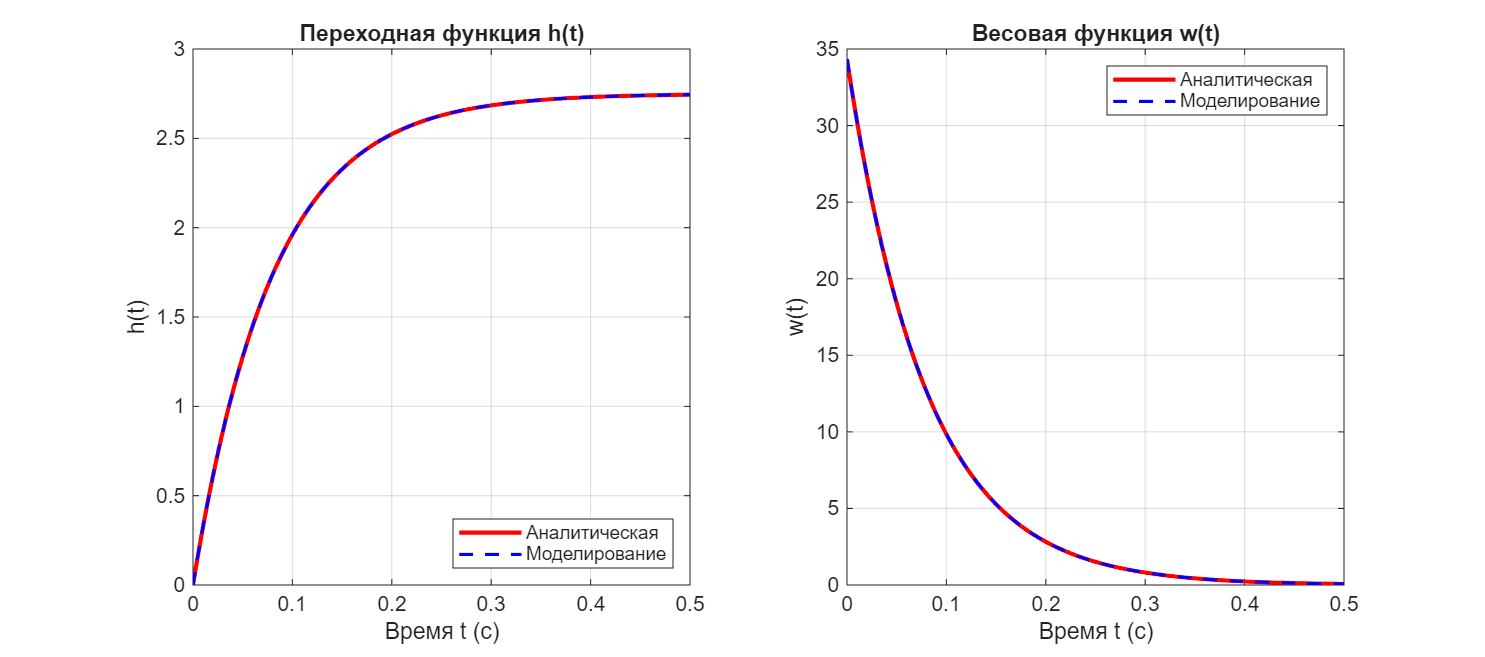
\includegraphics[width=0.95\textwidth]{obj1_time.png}
    \caption{Сравнительные графики переходной $h_1(t)$ и весовой $w_1(t)$ функций Объекта 1}
    \label{fig:obj1_time}
\end{figure}

\begin{figure}[H]
    \centering
    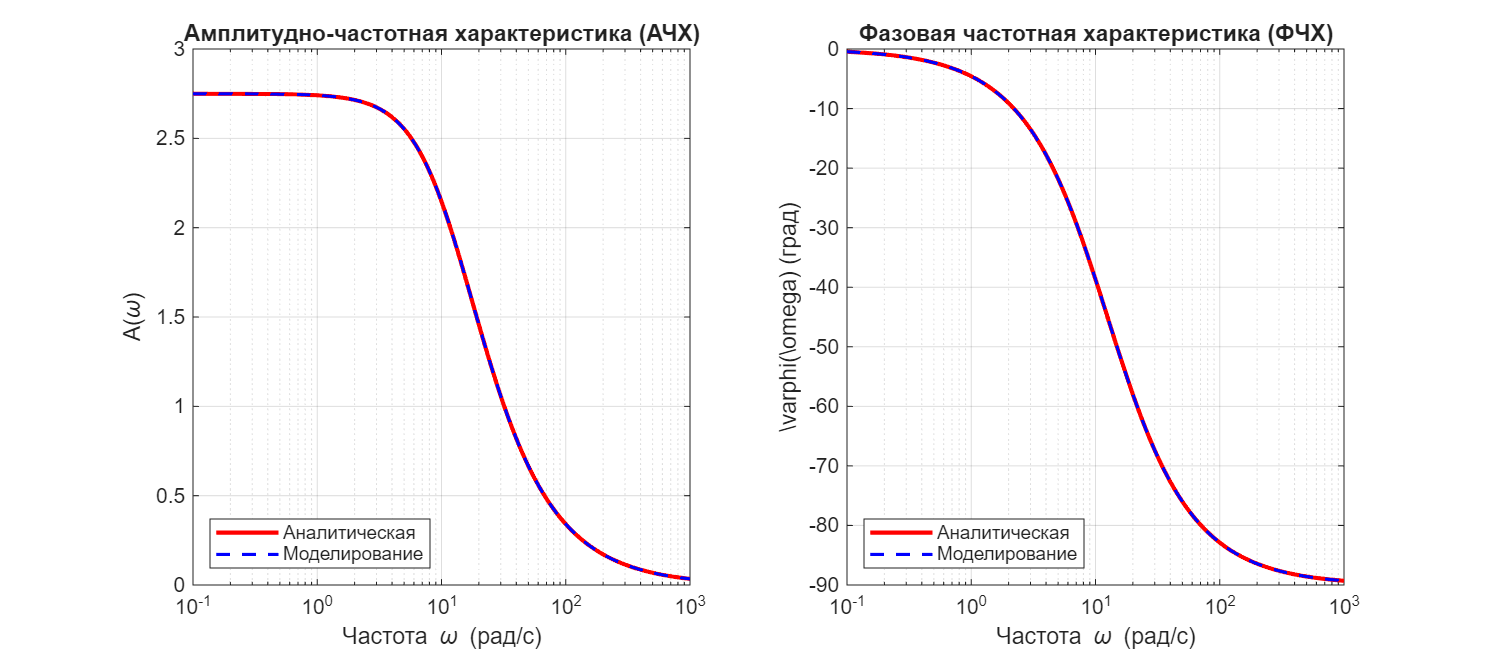
\includegraphics[width=0.95\textwidth]{obj1_freq.png}
    \caption{Сравнительные графики АЧХ и ФЧХ Объекта 1}
    \label{fig:obj1_freq}
\end{figure}

\begin{figure}[H]
    \centering
    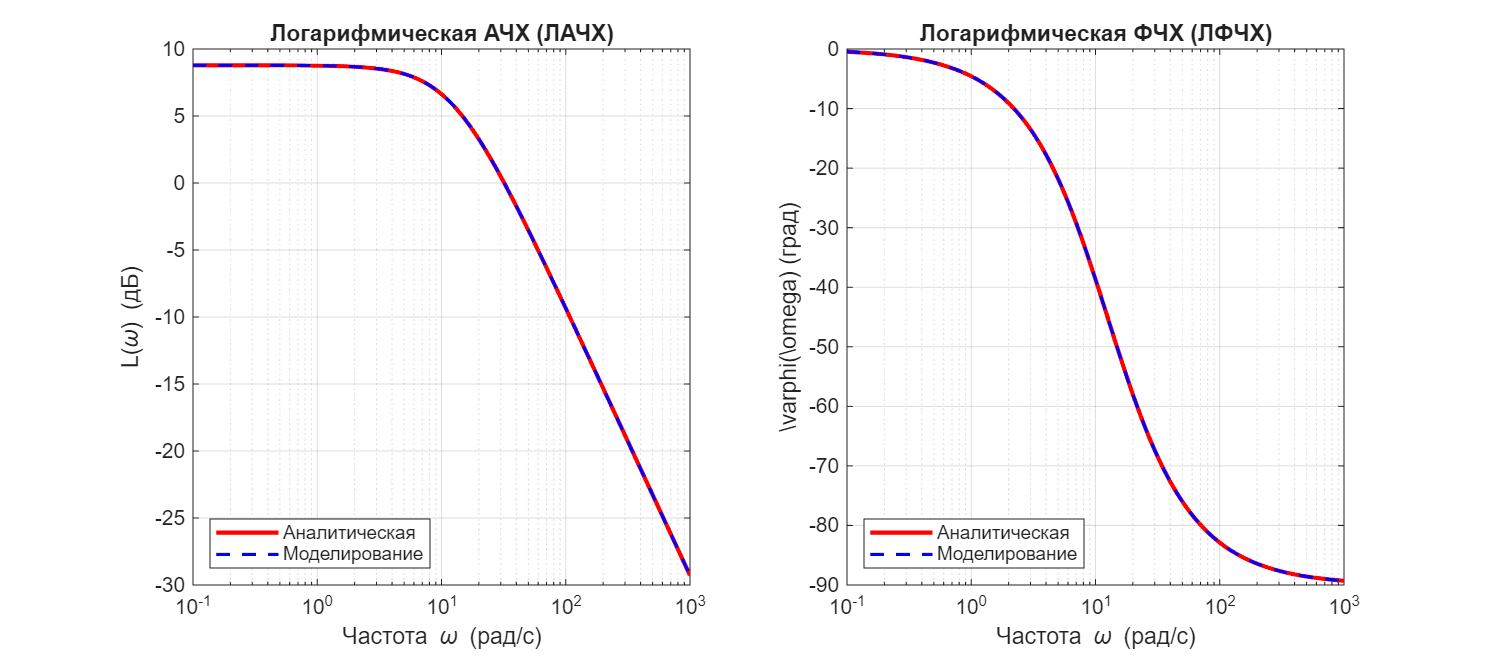
\includegraphics[width=0.95\textwidth]{obj1_bode.png}
    \caption{Сравнительные графики ЛАЧХ и ЛФЧХ Объекта 1}
    \label{fig:obj1_bode}
\end{figure}

По результатам моделирования видно полное совпадение кривых, построенных по аналитическим выражениям, и характеристик, полученных путем компьютерного моделирования в среде MATLAB:
\begin{itemize}
    \item Переходная характеристика $h_1(t)$ монотонно стремится от $0$ к установившемуся значению $K = 2.7495\text{ рад/с}$ без перерегулирования. Время переходного процесса (вхождение в $5\%$-ю зону) составляет $t_{\text{п}} \approx 3T \approx 0.240\text{ с}$.
    \item Весовая функция $w_1(t)$ в начальный момент времени максимальна и равна $\frac{K}{T} = 34.3387\text{ рад/(В}\cdot\text{с}^2)$, после чего экспоненциально затухает до нуля.
    \item На графике АЧХ максимальное усиление достигается при $\omega = 0$ и равно $A_1(0) = 2.7495$ ($L_1(0) = 8.7851\text{ дБ}$). С ростом частоты амплитуда монотонно убывает (высокочастотные сигналы подавляются, наклон ЛАЧХ после сопрягающей частоты $\omega_{\text{сопр}} = \frac{1}{T} = 12.489\text{ рад/с}$ составляет $-20\text{ дБ/дек}$). Частота среза (где $A_1(\omega_{\text{ср}}) = 1$, $L_1(\omega_{\text{ср}}) = 0\text{ дБ}$) равна $\omega_{\text{ср}} = \frac{\sqrt{K^2-1}}{T} \approx 32.02\text{ рад/с}$.
    \item Фазовый сдвиг $\varphi_1(\omega)$ изменяется от $0^\circ$ при $\omega = 0$ до $-90^\circ$ ($-\frac{\pi}{2}\text{ рад}$) при $\omega \to \infty$, принимая значение $-45^\circ$ на сопрягающей частоте $\omega = \frac{1}{T} = 12.489\text{ рад/с}$.
\end{itemize}

% -----------------------------------------------------------
\subsection{Выводы по Объекту 1}

В ходе выполнения работы для двигателя постоянного тока независимого возбуждения без учета индуктивности якорной обмотки (Вариант 3) была выведена передаточная функция в стандартизированном виде $W_1(s) = \frac{2.7495}{0.0801s + 1}$, соответствующая апериодическому звену 1-го порядка. Получены аналитические выражения для переходной и весовой функций, а также для частотных характеристик (АЧХ, ФЧХ, ЛАЧХ, ЛФЧХ). Сравнительный анализ графиков показал полное совпадение аналитических расчетов с результатами компьютерного моделирования. Звено обладает свойствами фильтра нижних частот и характеризуется монотонным переходным процессом без колебаний.


\newpage
\section{Объект 2: Двигатель постоянного тока с учетом индуктивности}

\subsection{Передаточная функция объекта в стандартизированном виде и значения параметров}

\textbf{Исходные данные (Вариант 3):}

Динамика двигателя постоянного тока независимого возбуждения с учетом индуктивности якорной обмотки описывается следующей системой уравнений:
\begin{equation}
    J\dot{\omega} = M, \quad M = k_m I, \quad I = \frac{U + \varepsilon}{R}, \quad \varepsilon = \varepsilon_i + \varepsilon_s, \quad \varepsilon_i = -k_e\omega, \quad \varepsilon_s = -L\dot{I},
\end{equation}
где входом объекта является напряжение питания $U(t)$, а выходом — угловая скорость вращения ротора $\Omega(t)$.

Значения физических параметров для варианта 3 (из таблицы 2) приведены в таблице \ref{tab:obj2_params}.

\begin{table}[H]
\centering
\caption{Параметры Объекта 2 (Вариант 3)}
\label{tab:obj2_params}
\setlength{\tabcolsep}{10pt} 
\renewcommand{\arraystretch}{1.3} 
\begin{tabular}{@{} >{\raggedright\arraybackslash}p{3.5cm} >{\raggedright\arraybackslash}p{7.5cm} c @{}}
\toprule
\textbf{Обозначение} & \textbf{Наименование параметра} & \textbf{Значение} \\ \midrule
$k_m$ & Конструктивная постоянная по моменту, $\text{Н}\cdot\text{м/А}$ & $0.3637$ \\
$k_e$ & Конструктивная постоянная по ЭДС, $\text{В}\cdot\text{с}$ & $0.3637$ \\
$J$   & Момент инерции ротора, $\text{кг}\cdot\text{м}^2$ & $0.0023$ \\
$R$   & Активное сопротивление обмоток ротора, $\text{Ом}$ & $4.6050$ \\ 
$L$   & Индуктивность обмоток ротора, $\text{Гн}$ & $1.1784$ \\ \bottomrule
\end{tabular}
\end{table}


Исключая промежуточные переменные из исходной системы уравнений, запишем дифференциальное уравнение второго порядка, связывающее входное напряжение $U(t)$ и выходную скорость $\omega(t)$:
\begin{equation*}
    \frac{JL}{k_m k_e}\ddot{\omega}(t) + \frac{JR}{k_m k_e}\dot{\omega}(t) + \omega(t) = \frac{1}{k_e}U(t).
\end{equation*}
Применив преобразование Лапласа при нулевых начальных условиях и переходя к передаточной функции $W_2(s) = \frac{\Omega(s)}{U(s)}$, получаем стандартизированный вид колебательного звена:
\begin{equation}
    W_2(s) = \frac{K}{T^2s^2 + 2\xi Ts + 1},
\end{equation}
где коэффициент усиления $K$, постоянная времени $T$ и коэффициент затухания $\xi$ определяются выражениями:
\begin{equation*}
    K = \frac{1}{k_e}, \quad T = \sqrt{\frac{JL}{k_m k_e}}, \quad \xi = \frac{JR}{2T k_m k_e}.
\end{equation*}

\textbf{Расчет численных значений параметров и итоговая передаточная функция:}
\begin{align*}
    K &= \frac{1}{0.3637} \approx 2.7495 \text{ (рад/с)/В}, \\
    T &= \sqrt{\frac{0.0023 \cdot 1.1784}{0.3637^2}} \approx 0.1431 \text{ с}, \\
    \xi &= \frac{0.0023 \cdot 4.6050}{2 \cdot 0.14314 \cdot 0.3637^2}\approx 0.2797.
\end{align*}
\begin{equation}
    W_2(s) = \frac{2.7495}{0.0205s^2 + 0.0801s + 1}.
\end{equation}

\textbf{Определение типового звена:} \\
Так как коэффициент затухания находится в диапазоне $0 < \xi < 1$ ($\xi = 0.2797$), исследуемый объект представляет собой \textbf{колебательное звено 2-го порядка} (минимально-фазовое).

% -----------------------------------------------------------
\subsection{Аналитически рассчитанные временные и частотные характеристики}

\subsubsection{Временные характеристики ($t \ge 0$)}

Для расчета временных характеристик введем параметры свободных колебаний:
\begin{itemize}
    \item Частота затухающих колебаний: $\omega_{\text{д}} = \frac{\sqrt{1 - \xi^2}}{T} = \frac{\sqrt{1 - 0.2797^2}}{0.14314} \approx 6.7069 \text{ рад/с}$.
    \item Скорость затухания: $\sigma_{\text{д}} = \frac{\xi}{T} = \frac{0.2797}{0.14314} \approx 1.9540 \text{ с}^{-1}$.
    \item Начальный фазовый угол: $\varphi_0 = \arccos(\xi) = \arccos(0.2797) \approx 1.2873 \text{ рад}$.
\end{itemize}

\begin{enumerate}
    \item \textbf{Переходная функция $h(t)$:}
    \begin{equation}
    \begin{aligned}
        h_2(t) &= K\left(1 - \frac{e^{-\sigma_{\text{д}}t}}{\sqrt{1-\xi^2}}\sin(\omega_{\text{д}}t + \arccos(\xi))\right) \\
        &= 2.7495\left(1 - 1.0416e^{-1.9540t}\sin(6.7069t + 1.2873)\right).
    \end{aligned}
    \end{equation}
    \item \textbf{Весовая функция $w(t)$:}
    \begin{equation}
        w_2(t) = \frac{Ke^{-\sigma_{\text{д}}t}}{T\sqrt{1-\xi^2}}\sin(\omega_{\text{д}}t) = 19.9922e^{-1.9540t}\sin(6.7069t).
    \end{equation}
\end{enumerate}

\subsubsection{Частотные характеристики ($\omega \ge 0$)}

Подставляя $s = j\omega$ в передаточную функцию $W_2(s)$, получаем ЧПФ:
\begin{equation*}
    W_2(j\omega) = \frac{K}{(1 - T^2\omega^2) + j(2\xi T\omega)} = \frac{2.7495}{(1 - 0.0205\omega^2) + j(0.0801\omega)}.
\end{equation*}

Отсюда выводятся частотные характеристики:
\begin{enumerate}
    \item \textbf{Амплитудно-частотная характеристика (АЧХ):}
    \begin{equation}
        A_2(\omega) = \frac{K}{\sqrt{(1 - T^2\omega^2)^2 + (2\xi T\omega)^2}} = \frac{2.7495}{\sqrt{(1 - 0.0205\omega^2)^2 + (0.0801\omega)^2}}.
    \end{equation}

    \item \textbf{Фазовая частотная характеристика (ФЧХ):}
    \begin{equation}
        \varphi_2(\omega) = -\text{arctg}\left(\frac{2\xi T\omega}{1 - T^2\omega^2}\right).
    \end{equation}

    \item \textbf{Логарифмическая амплитудная частотная характеристика (ЛАЧХ):}
    \begin{equation}
        L_2(\omega) = 20\lg A_2(\omega) = 8.7851 - 10\lg\left((1 - 0.0205\omega^2)^2 + (0.0801\omega)^2\right)\text{ (дБ)}.
    \end{equation}

    \item \textbf{Логарифмическая фазовая частотная характеристика (ЛФЧХ):} \\
    Совпадает с ФЧХ $\varphi_2(\omega)$, отображаемой в полулогарифмическом масштабе по оси частот.
\end{enumerate}

% -----------------------------------------------------------
\subsection{Графическое представление характеристик и сравнение с аналитическими результатами}

\begin{figure}[H]
    \centering
    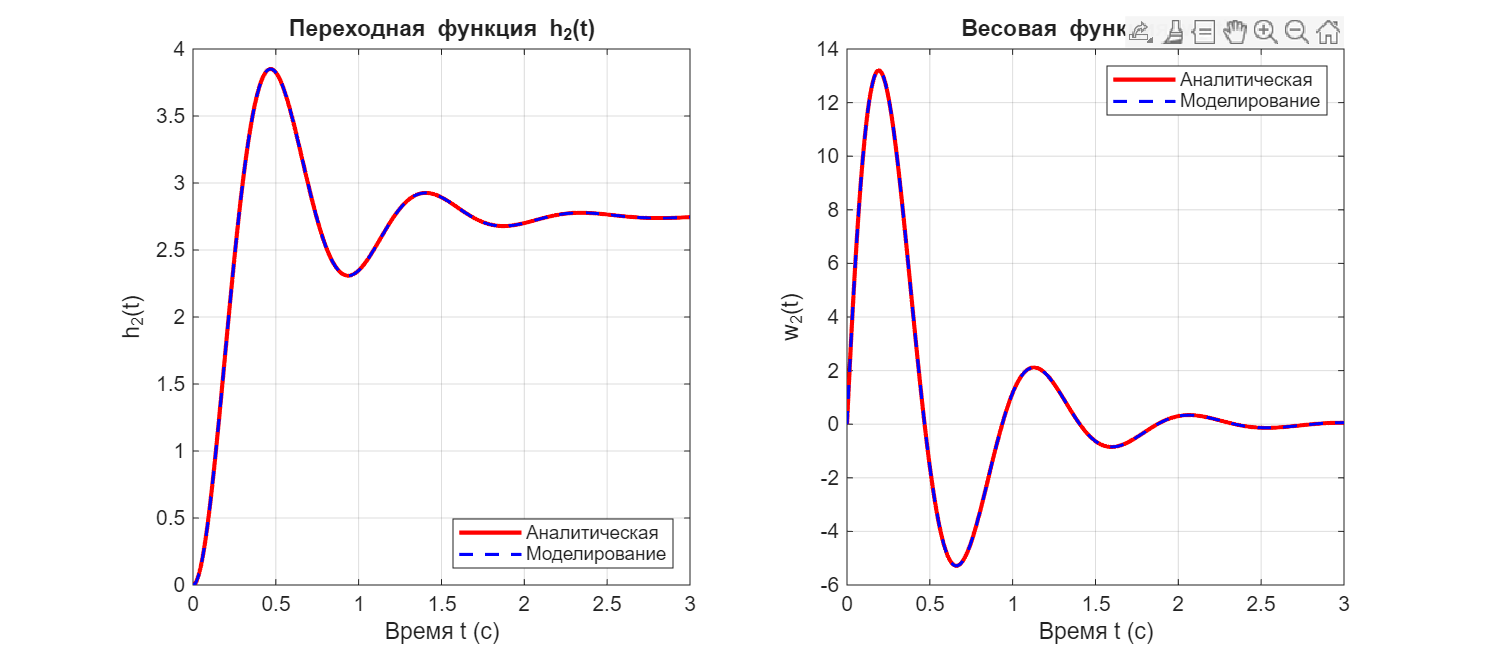
\includegraphics[width=0.85\textwidth]{obj2_time.png}
    \caption{Сравнительные графики переходной $h_2(t)$ и весовой $w_2(t)$ функций Объекта 2}
    \label{fig:obj2_time}
\end{figure}

\begin{figure}[H]
    \centering
    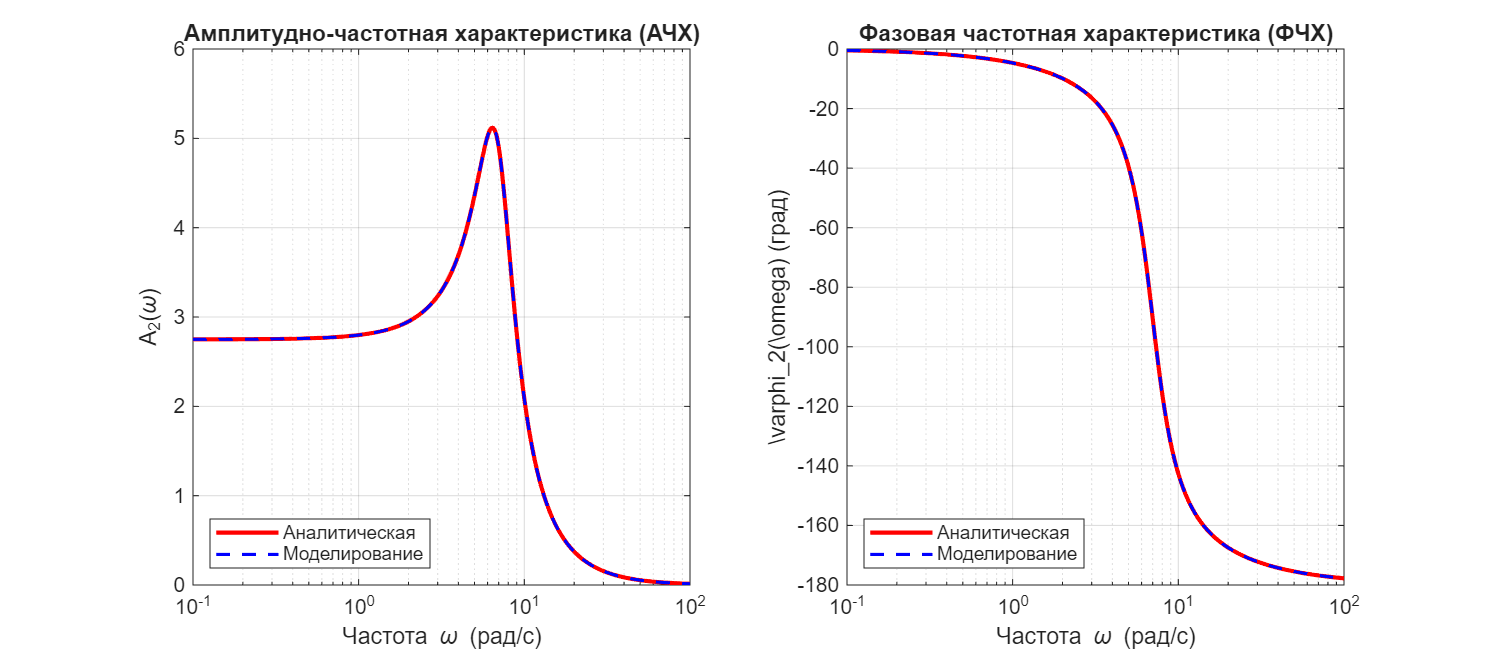
\includegraphics[width=0.85\textwidth]{obj2_freq.png}
    \caption{Сравнительные графики АЧХ и ФЧХ Объекта 2}
    \label{fig:obj2_freq}
\end{figure}

\begin{figure}[H]
    \centering
    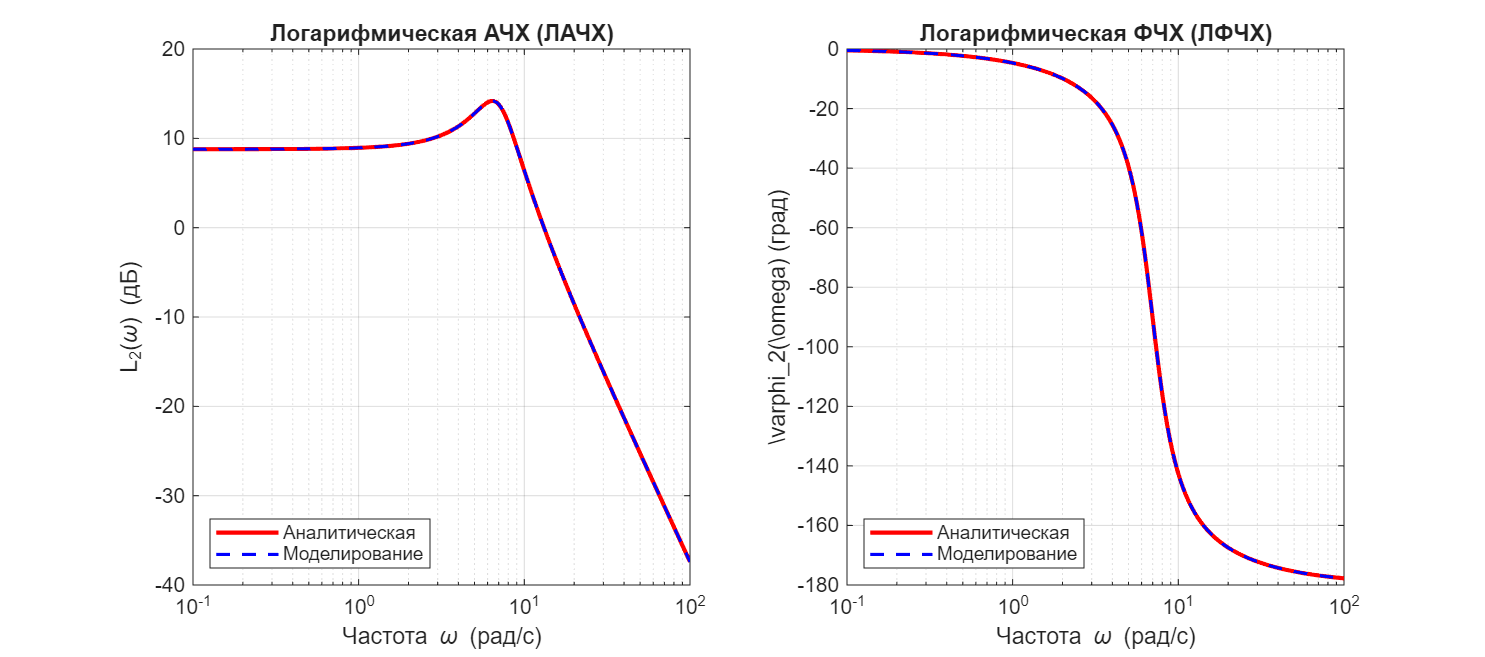
\includegraphics[width=0.85\textwidth]{obj2_bode.png}
    \caption{Сравнительные графики ЛАЧХ и ЛФЧХ Объекта 2}
    \label{fig:obj2_bode}
\end{figure}

По результатам моделирования наблюдается полное совпадение аналитических кривых с результатами компьютерного моделирования в MATLAB:
\begin{itemize}
    \item Переходная характеристика $h_2(t)$ носит колебательный характер с небольшим перерегулированием из-за малой величины коэффициента затухания ($\xi = 0.2797$), после чего плавно выходит на установившееся значение $2.7495\text{ рад/с}$.
    \item Весовая функция $w_2(t)$ представляет собой затухающие синусоидальные колебания.
    \item На графике АЧХ наблюдается резонансный пик на частоте $\omega_p \approx \frac{\sqrt{1-2\xi^2}}{T} \approx 6.42\text{ рад/с}$, что характерно для колебательных систем.
    \item ФЧХ изменяется в диапазоне от $0^\circ$ до $-180^\circ$.
\end{itemize}





% -----------------------------------------------------------
\subsection{Выводы по Объекту 2}

Для двигателя постоянного тока с учетом индуктивности якорной цепи (Вариант 3) получена передаточная функция колебательного звена 2-го порядка. Выведены аналитические зависимости временных и частотных характеристик с учетом коэффициента затухания $\xi = 0.2797$. Сопоставление аналитических расчетов с результатами моделирования в MATLAB подтвердило их высокую точность и правильность выводов теории автоматического управления.


\newpage
\section{Объект 3: Конденсатор}

\subsection{Передаточная функция объекта в стандартизированном виде и значения параметров}

\textbf{Исходные данные (Вариант 3):}

Уравнение электрического состояния конденсатора имеет вид:
\begin{equation}
    I(t) = C \frac{dU(t)}{dt},
\end{equation}
где входом объекта является ток $I(t)$, а выходом — напряжение на конденсаторе $U(t)$.

Значение емкости конденсатора для варианта 3 (из таблицы 3) приведено в таблице \ref{tab:obj3_params}.

\begin{table}[H]
\centering
\caption{Параметры Объекта 3 (Вариант 3)}
\label{tab:obj3_params}
\setlength{\tabcolsep}{10pt} 
\renewcommand{\arraystretch}{1.3} 
\begin{tabular}{@{} >{\raggedright\arraybackslash}p{3.5cm} >{\raggedright\arraybackslash}p{7.5cm} c @{}}
\toprule
\textbf{Обозначение} & \textbf{Наименование параметра} & \textbf{Значение} \\ \midrule
$C$ & Емкость конденсатора, $\text{мкФ}$ & $287$ ($287 \cdot 10^{-6} \text{ Ф}$) \\ \bottomrule
\end{tabular}
\end{table}

\textbf{Вывод передаточной функции:}

Применив преобразование Лапласа к исходному дифференциальному уравнению при нулевых начальных условиях ($U(0) = 0$), получаем операторное уравнение:
\begin{equation*}
    I(s) = C s U(s) \implies U(s) = \frac{1}{Cs} I(s).
\end{equation*}
Отсюда передаточная функция объекта принимает вид идеального интегрирующего звена:
\begin{equation}
    W_3(s) = \frac{U(s)}{I(s)} = \frac{K}{s},
\end{equation}
где коэффициент усиления $K$ определяется выражением:
\begin{equation*}
    K = \frac{1}{C}.
\end{equation*}

\textbf{Расчет численного значения параметра и итоговая передаточная функция:}
\begin{align*}
    K &= \frac{1}{287 \cdot 10^{-6}} \approx 3484.3206 \text{ Ф}^{-1}.
\end{align*}
\begin{equation}
    W_3(s) = \frac{3484.3206}{s}.
\end{equation}

\textbf{Определение типового звена:} \\
По виду полученной передаточной функции исследуемый объект представляет собой \textbf{идеальное интегрирующее звено}.

% -----------------------------------------------------------
\subsection{Аналитически рассчитанные временные и частотные характеристики}

\subsubsection{Временные характеристики ($t \ge 0$)}

\begin{enumerate}
    \item \textbf{Переходная функция $h(t)$:}
    \begin{equation}
        h_3(t) = \mathcal{L}^{-1}\left\{\frac{W_3(s)}{s}\right\} = Kt = 3484.3206t.
    \end{equation}

    \item \textbf{Весовая функция $w(t)$:}
    \begin{equation}
        w_3(t) = \mathcal{L}^{-1}\{W_3(s)\} = K = 3484.3206.
    \end{equation}
\end{enumerate}

\subsubsection{Частотные характеристики ($\omega \ge 0$)}

Подставляя $s = j\omega$ в передаточную функцию, получаем частотную передаточную функцию:
\begin{equation*}
    W_3(j\omega) = \frac{K}{j\omega} = -j\frac{K}{\omega}.
\end{equation*}

Отсюда выводятся частотные характеристики:
\begin{enumerate}
    \item \textbf{Амплитудно-частотная характеристика (АЧХ):}
    \begin{equation}
        A_3(\omega) = \frac{K}{\omega} = \frac{3484.3206}{\omega}.
    \end{equation}

    \item \textbf{Фазовая частотная характеристика (ФЧХ):}
    \begin{equation}
        \varphi_3(\omega) = -\frac{\pi}{2} = -90^\circ \text{ (const)}.
    \end{equation}

    \item \textbf{Логарифмическая амплитудная частотная характеристика (ЛАЧХ):}
    \begin{equation}
        L_3(\omega) = 20\lg A_3(\omega) = 20\lg K - 20\lg\omega = 70.8424 - 20\lg\omega \text{ (дБ)}.
    \end{equation}

    \item \textbf{Логарифмическая фазовая частотная характеристика (ЛФЧХ):} \\
    Содержит постоянное значение $-90^\circ$ во всем диапазоне частот $\omega$.
\end{enumerate}

% -----------------------------------------------------------
\subsection{Графическое представление характеристик и сравнение с аналитическими результатами}

\begin{figure}[H]
    \centering
    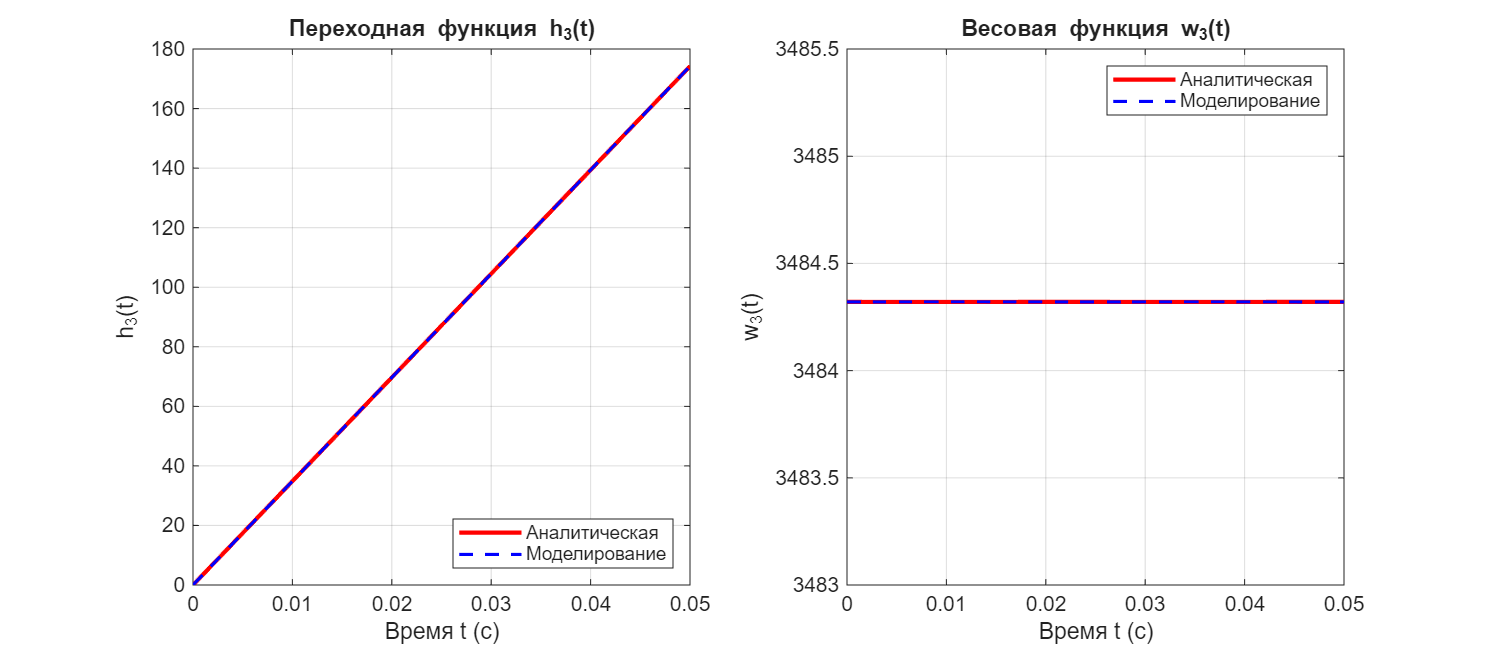
\includegraphics[width=0.85\textwidth]{obj3_time.png}
    \caption{Сравнительные графики переходной $h_3(t)$ и весовой $w_3(t)$ функций Объекта 3}
    \label{fig:obj3_time}
\end{figure}

\begin{figure}[H]
    \centering
    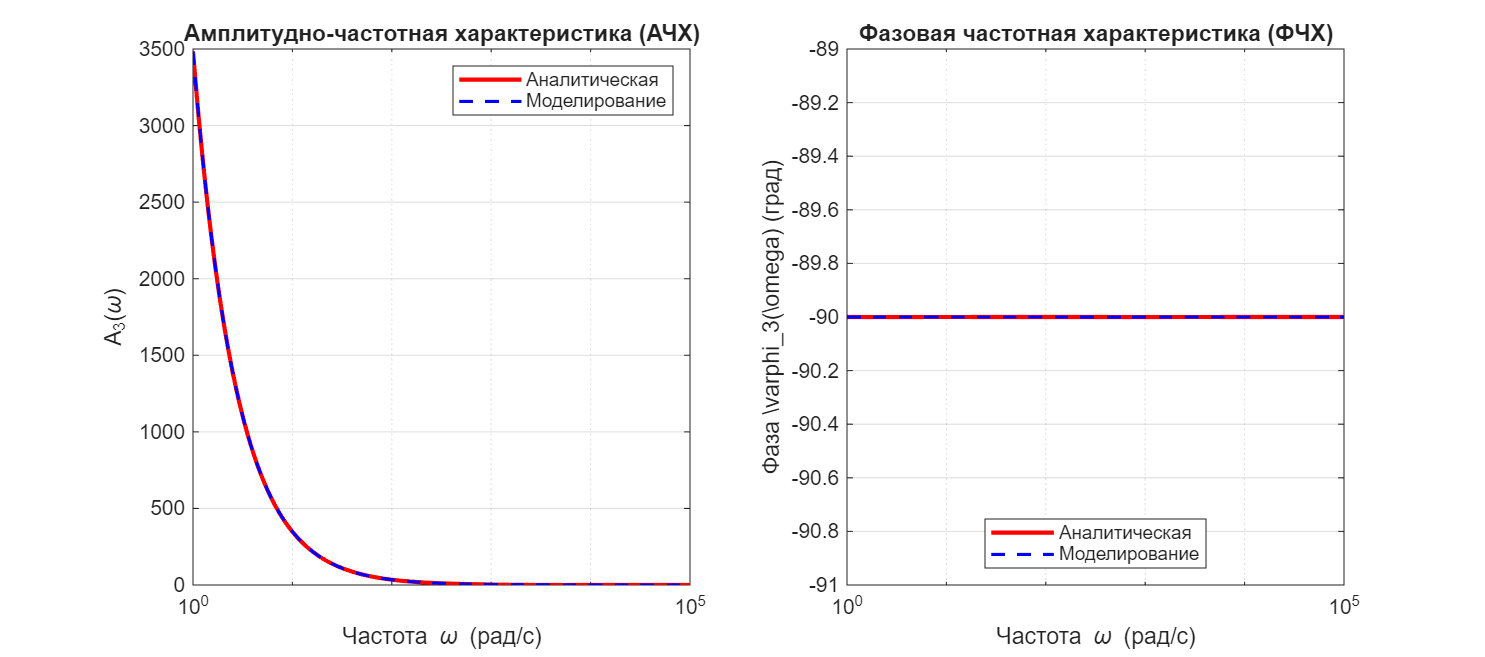
\includegraphics[width=0.85\textwidth]{obj3_freq.png}
    \caption{Сравнительные графики АЧХ и ФЧХ Объекта 3}
    \label{fig:obj3_freq}
\end{figure}

\begin{figure}[H]
    \centering
    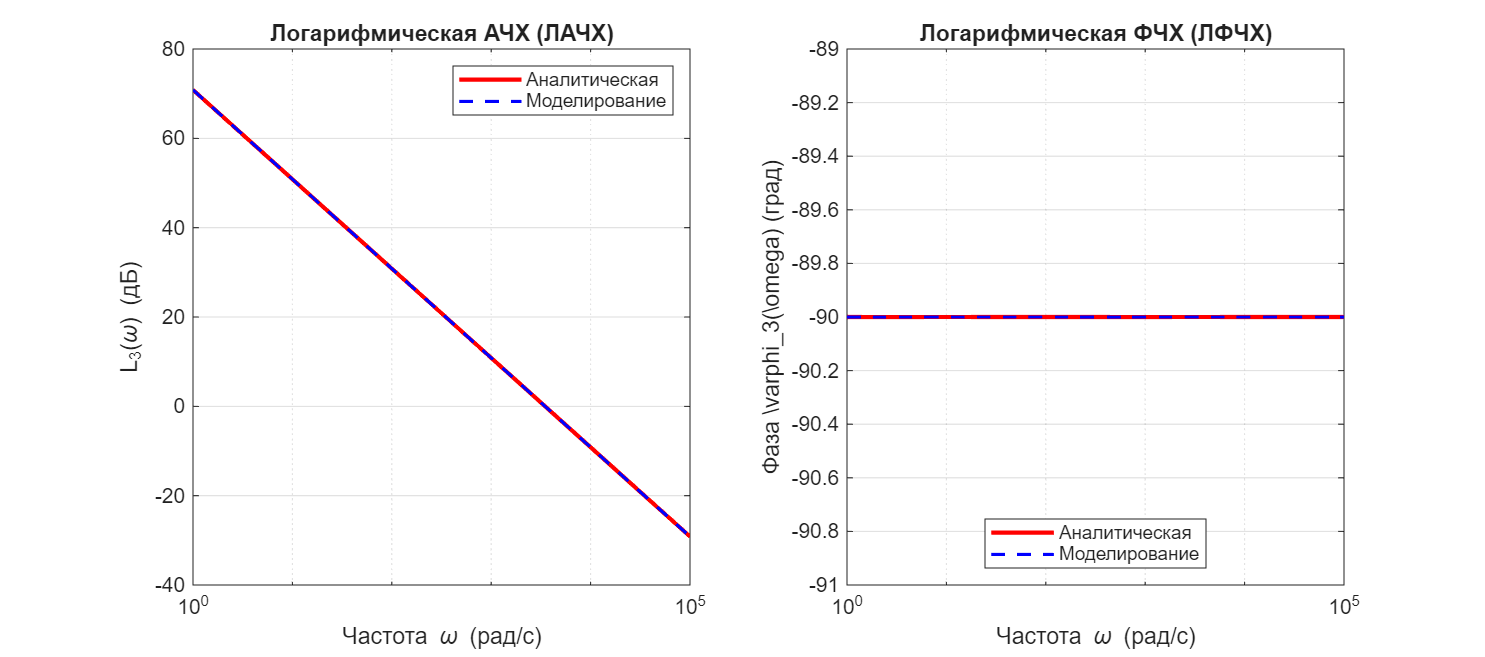
\includegraphics[width=0.85\textwidth]{obj3_bode.png}
    \caption{Сравнительные графики ЛАЧХ и ЛФЧХ Объекта 3}
    \label{fig:obj3_bode}
\end{figure}

По результатам моделирования наблюдается полное совпадение аналитических кривых с результатами компьютерного моделирования в MATLAB:
\begin{itemize}
    \item Переходная характеристика $h_3(t)$ представляет собой линейно возрастающую функцию с постоянной скоростью роста, определяемой коэффициентом $K$.
    \item Весовая функция $w_3(t)$ является постоянной величиной, равной $K$.
    \item АЧХ монотонно убывает с ростом частоты, а ЛАЧХ представляет собой прямую линию с постоянным наклоном $-20\text{ дБ/дек}$.
    \item ФЧХ тождественно равна $-90^\circ$ на всех частотах.
\end{itemize}




% -----------------------------------------------------------
\subsection{Выводы по Объекту 3}

Для конденсатора (Вариант 3) получена передаточная функция идеального интегрирующего звена с коэффициентом усиления $K \approx 3484.3206\text{ Ф}^{-1}$. Выведены аналитические зависимости временных и частотных характеристик. Сопоставление с результатами моделирования в MATLAB показало их полное совпадение. Звено осуществляет операцию интегрирования входного тока, что подтверждается линейным ростом напряжения на выходе.

\newpage
\section{Объект 4: Пружина}

\subsection{Передаточная функция объекта в стандартизированном виде и значения параметров}

\textbf{Исходные данные (Вариант 3):}

Динамика пружинного маятника (консервативной механической системы) описывается вторым законом Ньютона с учетом упругой силы пружины:
\begin{equation}
    M\ddot{x}(t) = F_{\text{вн}}(t) + F_{\text{упр}}, \quad F_{\text{упр}} = -kx,
\end{equation}
где входом объекта является внешняя сила $F_{\text{вн}}(t)$, а выходом — перемещение груза $x(t)$.

Значения массы груза и коэффициента жесткости пружины для варианта 3 (из таблицы 4) приведены в таблице \ref{tab:obj4_params}.

\begin{table}[H]
\centering
\caption{Параметры Объекта 4 (Вариант 3)}
\label{tab:obj4_params}
\setlength{\tabcolsep}{10pt} 
\renewcommand{\arraystretch}{1.3} 
\begin{tabular}{@{} >{\raggedright\arraybackslash}p{3.5cm} >{\raggedright\arraybackslash}p{7.5cm} c @{}}
\toprule
\textbf{Обозначение} & \textbf{Наименование параметра} & \textbf{Значение} \\ \midrule
$M$ & Масса груза, $\text{кг}$ & $13$ \\
$k$ & Коэффициент жесткости пружины, $\text{Н/м}$ & $322$ \\ \bottomrule
\end{tabular}
\end{table}

\textbf{Вывод передаточной функции:}

Подставим силу упругости в уравнение движения:
\begin{equation*}
    M\ddot{x}(t) + kx(t) = F_{\text{вн}}(t).
\end{equation*}
Разделив обе части уравнения на жесткость $k$, приведем его к стандартизированному виду:
\begin{equation*}
    \frac{M}{k}\ddot{x}(t) + x(t) = \frac{1}{k}F_{\text{вн}}(t).
\end{equation*}
Применив преобразование Лапласа при нулевых начальных условиях и переходя к передаточной функции $W_4(s) = \frac{x(s)}{F_{\text{вн}}(s)}$, получаем стандартизированный вид консервативного звена:
\begin{equation}
    W_4(s) = \frac{K}{T^2s^2 + 1},
\end{equation}
где коэффициент усиления $K$ и постоянная времени $T$ определяются выражениями:
\begin{equation*}
    K = \frac{1}{k}, \quad T = \sqrt{\frac{M}{k}}.
\end{equation*}

\textbf{Расчет численных значений параметров и итоговая передаточная функция:}
\begin{align*}
    K &= \frac{1}{322} \approx 0.003106 \text{ м/Н}, \\
    T &= \sqrt{\frac{13}{322}} = \sqrt{0.040373} \approx 0.2009 \text{ с}.
\end{align*}
\begin{equation}
    W_4(s) = \frac{0.003106}{0.04037s^2 + 1}.
\end{equation}

\textbf{Определение типового звена:} \\
По виду полученной передаточной функции исследуемый объект представляет собой \textbf{консервативное звено} (частный случай колебательного звена при нулевом затухании $\xi = 0$).

% -----------------------------------------------------------
\subsection{Аналитически рассчитанные временные и частотные характеристики}

\subsubsection{Временные характеристики ($t \ge 0$)}

\begin{enumerate}
    \item \textbf{Переходная функция $h(t)$:}
    \begin{equation}
        h_4(t) = K\left(1 - \cos\left(\frac{t}{T}\right)\right) = 0.003106\left(1 - \cos(4.9769t)\right).
    \end{equation}

    \item \textbf{Весовая функция $w(t)$:}
    \begin{equation}
        w_4(t) = \frac{K}{T}\sin\left(\frac{t}{T}\right) = 0.01546\sin(4.9769t).
    \end{equation}
\end{enumerate}

\subsubsection{Частотные характеристики ($\omega \ge 0$)}

Подставляя $s = j\omega$ в передаточную функцию, получаем частотную передаточную функцию:
\begin{equation*}
    W_4(j\omega) = \frac{K}{1 - T^2\omega^2} = \frac{0.003106}{1 - 0.04037\omega^2}.
\end{equation*}

Отсюда выводятся частотные характеристики:
\begin{enumerate}
    \item \textbf{Амплитудно-частотная характеристика (АЧХ):}
    \begin{equation}
        A_4(\omega) = \frac{K}{|1 - T^2\omega^2|} = \frac{0.003106}{|1 - 0.04037\omega^2|}.
    \end{equation}
    *(Примечание: на резонансной частоте $\omega_p = \frac{1}{T} \approx 4.9769\text{ рад/с}$ АЧХ стремится к бесконечности из-за отсутствия затухания).*

    \item \textbf{Фазовая частотная характеристика (ФЧХ):}
    \begin{equation}
        \varphi_4(\omega) = \begin{cases} 
            0^\circ, & \omega < \frac{1}{T} \\ 
            -180^\circ, & \omega > \frac{1}{T}
        \end{cases}
    \end{equation}

    \item \textbf{Логарифмическая амплитудная частотная характеристика (ЛАЧХ):}
    \begin{equation}
        L_4(\omega) = 20\lg A_4(\omega) = -50.148 - 20\lg|1 - 0.04037\omega^2|\text{ (дБ)}.
    \end{equation}

    \item \textbf{Логарифмическая фазовая частотная характеристика (ЛФЧХ):} \\
    Имеет скачкообразное изменение фазы на $-180^\circ$ при прохождении резонансной частоты $\omega_p \approx 4.9769\text{ рад/с}$.
\end{enumerate}

% -----------------------------------------------------------
\subsection{Графическое представление характеристик и сравнение с аналитическими результатами}

\begin{figure}[H]
    \centering
    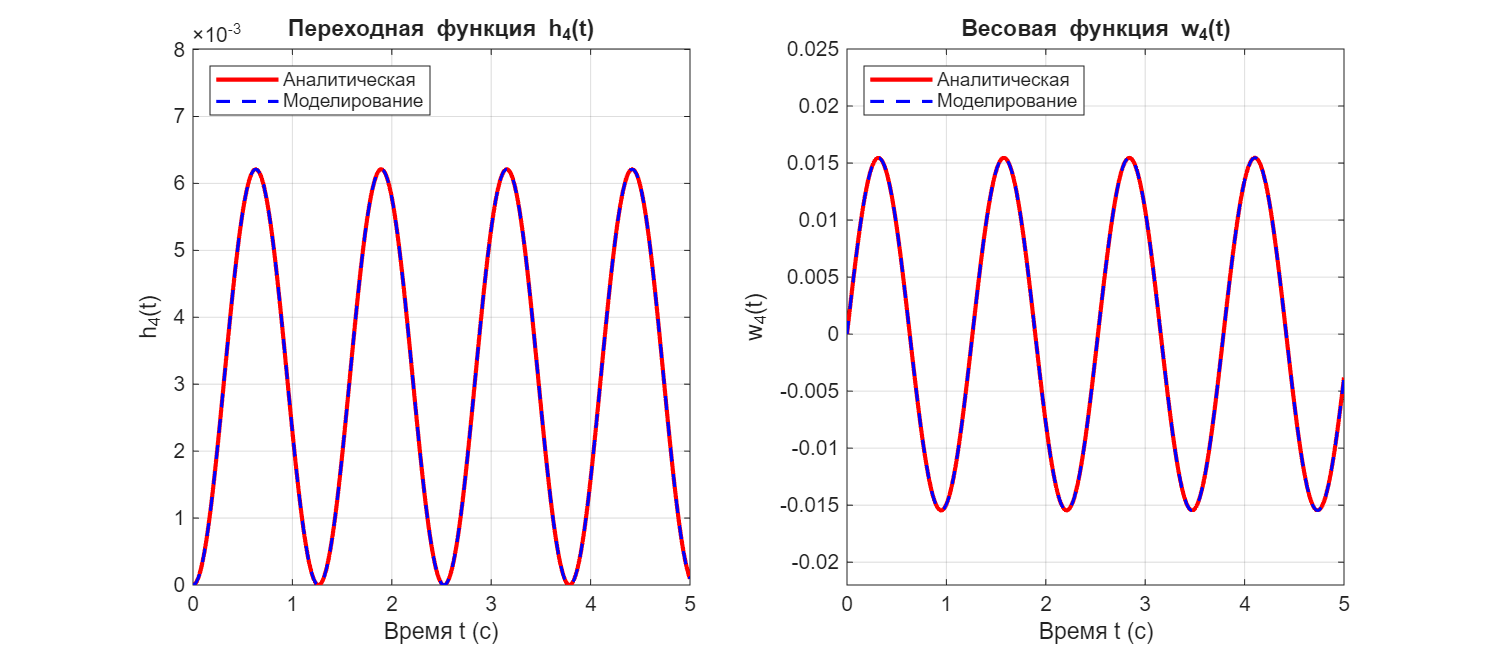
\includegraphics[width=0.85\textwidth]{obj4_time.png}
    \caption{Сравнительные графики переходной $h_4(t)$ и весовой $w_4$ функций Объекта 4}
    \label{fig:obj4_time}
\end{figure}

\begin{figure}[H]
    \centering
    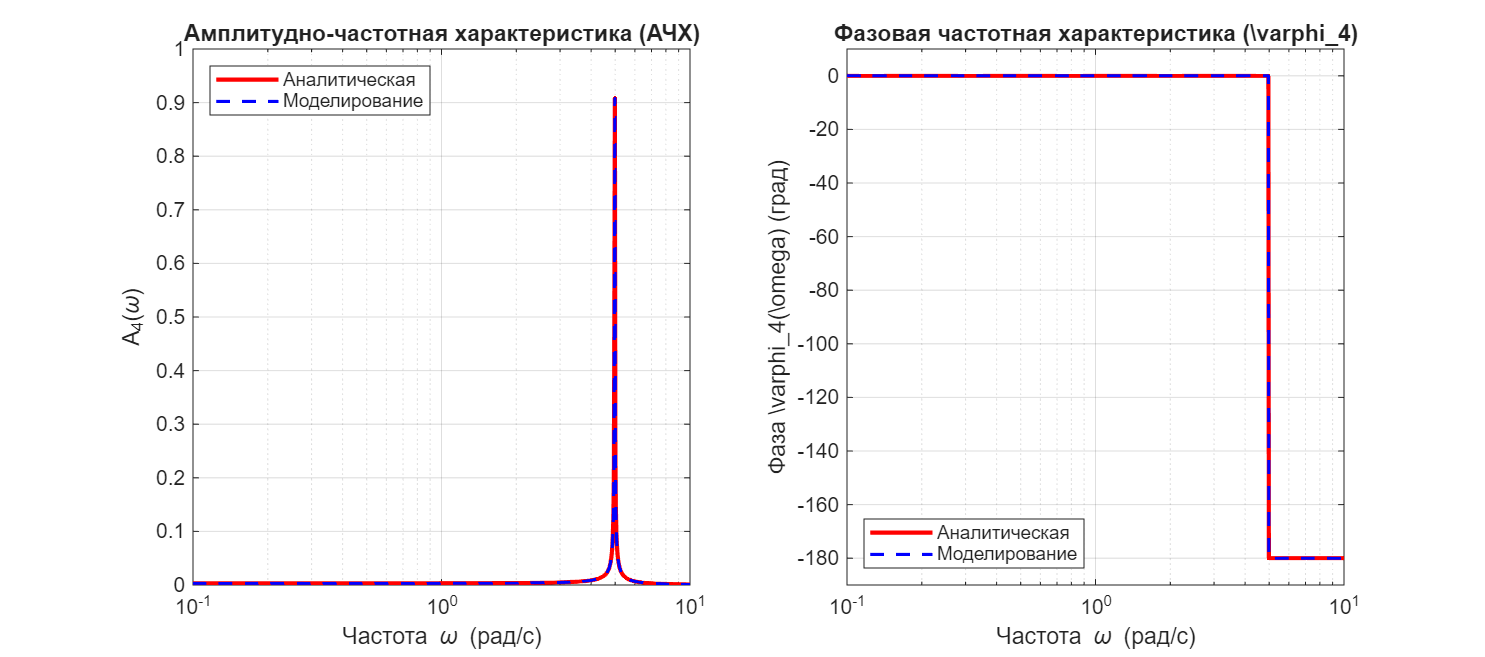
\includegraphics[width=0.85\textwidth]{obj4_freq.png}
    \caption{Сравнительные графики АЧХ и ФЧХ Объекта 4}
    \label{fig:obj4_freq}
\end{figure}

\begin{figure}[H]
    \centering
    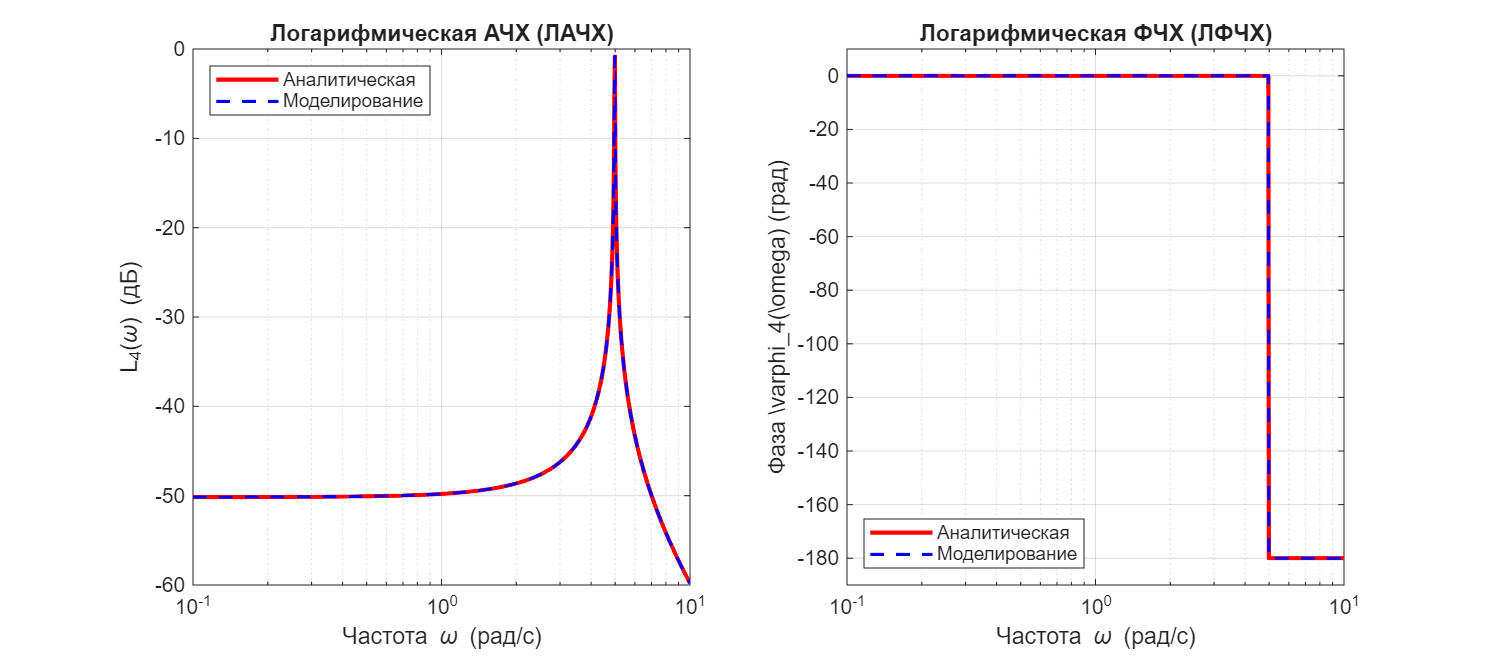
\includegraphics[width=0.85\textwidth]{obj4_bode.png}
    \caption{Сравнительные графики ЛАЧХ и ЛФЧХ Объекта 4}
    \label{fig:obj4_bode}
\end{figure}

По результатам моделирования наблюдается полное совпадение аналитических кривых с результатами компьютерного моделирования в MATLAB:
\begin{itemize}
    \item Переходная характеристика $h_4(t)$ представляет собой незатухающие гармонические колебания около постоянного уровня.
    \item Весовая функция $w_4(t)$ также имеет вид незатухающих синусоидальных колебаний.
    \item На частотных характеристиках в точке резонанса ($ \approx 4.9769\text{ рад/с}$) наблюдается резкий пик амплитуды и скачок фазы на $-180^\circ$, что обусловлено консервативным характером системы (отсутствием диссипации энергии).
\end{itemize}


\subsection{Выводы по Объекту 4}

Для пружинного маятника (Вариант 3) получена передаточная функция консервативного звена с параметрами $K \approx 0.003106\text{ м/Н}$ и $T \approx 0.2009\text{ с}$. Выведены аналитические зависимости для характеристик во временной и частотной областях. Ввиду отсутствия диссипации энергии ($\xi = 0$), система демонстрирует незатухающие колебания во времени и бесконечный резонансный пик на частоте $\approx 4.9769\text{ рад/с}$, что полностью подтверждено результатами моделирования в MATLAB.



\newpage
\section{Объект 5: Операционный усилитель}

\subsection{Передаточная функция объекта в стандартизированном виде и значения параметров}

\textbf{Исходные данные (Вариант 3):}

Схема регулятора на операционном усилителе (рисунок 16) имеет входной резистор $R_1$ и цепь отрицательной обратной связи, состоящую из последовательно соединенных конденсатора $C$ и резистора $R_2$[cite: 48, 49]. Входным сигналом является $U_{\text{вх}}(t)$, а выходным — $U_{\text{вых}}(t)$[cite: 48]. Знак инверсии в рамках задания не учитывается (берется модуль коэффициента усиления)[cite: 48].

Значения параметров для варианта 3 (из таблицы 5) приведены в таблице \ref{tab:obj5_params}[cite: 46].

\begin{table}[H]
\centering
\caption{Параметры Объекта 5 (Вариант 3)}
\label{tab:obj5_params}
\setlength{\tabcolsep}{10pt} 
\renewcommand{\arraystretch}{1.3} 
\begin{tabular}{@{} >{\raggedright\arraybackslash}p{3.5cm} >{\raggedright\arraybackslash}p{7.5cm} c @{}}
\toprule
\textbf{Обозначение} & \textbf{Наименование параметра} & \textbf{Значение} \\ \midrule
$R_1$ & Сопротивление входного резистора, $\text{Ом}$ & $917$[cite: 46] \\
$R_2$ & Сопротивление резистора обратной связи, $\text{Ом}$ & $14665$[cite: 46] \\
$C$   & Емкость конденсатора обратной связи, $\text{мкФ}$ & $287$ ($287 \cdot 10^{-6} \text{ Ф}$)[cite: 46] \\ \bottomrule
\end{tabular}
\end{table}

\textbf{Вывод передаточной функции:}

Передаточная функция неинвертирующего/инвертирующего усилителя по модулю определяется отношением импеданса цепи обратной связи $Z_{\text{ос}}(s) = R_2 + \frac{1}{Cs} = \frac{R_2Cs + 1}{Cs}$ к входному сопротивлению $Z_1(s) = R_1$:
\begin{equation*}
    W_5(s) = \left| -\frac{Z_{\text{ос}}(s)}{Z_1(s)} \right| = \frac{R_2Cs + 1}{R_1Cs} = \frac{R_2}{R_1}\left(1 + \frac{1}{R_2Cs}\right).
\end{equation*}
Приведя к стандартизированному виду изодромного интегрирующего звена, получаем:
\begin{equation}
    W_5(s) = K \frac{Ts + 1}{s},
\end{equation}
где коэффициент усиления $K$ и постоянная времени $T$ равны:
\begin{equation*}
    K = \frac{1}{R_1 C}, \quad T = R_2 C.
\end{equation*}

\textbf{Расчет численных значений параметров и итоговая передаточная функция:}
\begin{align*}
    K &= \frac{1}{917 \cdot 287 \cdot 10^{-6}} = \frac{1}{0.263179} \approx 3.7997 \text{ с}^{-1}, \\
    T &= 14665 \cdot 287 \cdot 10^{-6} \approx 4.2089 \text{ с}.
\end{align*}
\begin{equation}
    W_5(s) = 3.7997 \frac{4.2089s + 1}{s}.
\end{equation}

\textbf{Определение типового звена:} \\
Исследуемый объект представляет собой \textbf{изодромное интегрирующее звено} (ПИ-регулятор).

% -----------------------------------------------------------
\subsection{Аналитически рассчитанные временные и частотные характеристики}

\subsubsection{Временные характеристики ($t \ge 0$)}

\begin{enumerate}
    \item \textbf{Переходная функция $h(t)$:}
    \begin{equation}
        h_5(t) = K(T + t) = 3.7997(4.2089 + t) = 15.9924 + 3.7997t.
    \end{equation}

    \item \textbf{Весовая функция $w(t)$:}
    \begin{equation}
        w_5(t) = KT\delta(t) + K = 15.9924\delta(t) + 3.7997.
    \end{equation}
    *(Примечание: при компьютерном моделировании и построении графиков весовой функции гармоническая составляющая $\delta(t)$ опускается).*
\end{enumerate}

\subsubsection{Частотные характеристики ($\omega \ge 0$)}

Подставляя $s = j\omega$, получаем частотную передаточную функцию:
\begin{equation*}
    W_5(j\omega) = K \frac{1 + j\omega T}{j\omega} = KT - j\frac{K}{\omega}.
\end{equation*}

Отсюда выводятся частотные характеристики:
\begin{enumerate}
    \item \textbf{Амплитудно-частотная характеристика (АЧХ):}
    \begin{equation}
        A_5(\omega) = \frac{K\sqrt{1 + (\omega T)^2}}{\omega} = \frac{3.7997\sqrt{1 + (4.2089\omega)^2}}{\omega}.
    \end{equation}

    \item \textbf{Фазовая частотная характеристика (ФЧХ):}
    \begin{equation}
        \varphi_5(\omega) = -\frac{\pi}{2} + \text{arctg}(\omega T) = -90^\circ + \text{arctg}(4.2089\omega) \text{ (град)}.
    \end{equation}

    \item \textbf{Логарифмическая амплитудная частотная характеристика (ЛАЧХ):}
    \begin{equation}
        L_5(\omega) = 20\lg A_5(\omega) = 20\lg K + 20\lg\sqrt{1 + (\omega T)^2} - 20\lg\omega \text{ (дБ)}.
    \end{equation}

    \item \textbf{Логарифмическая фазовая частотная характеристика (ЛФЧХ):} \\
    Совпадает с ФЧХ $\varphi_5(\omega)$, отображаемой в полулогарифмическом масштабе.
\end{enumerate}

% -----------------------------------------------------------
\subsection{Графическое представление характеристик и сравнение с аналитическими результатами}

\begin{figure}[H]
    \centering
    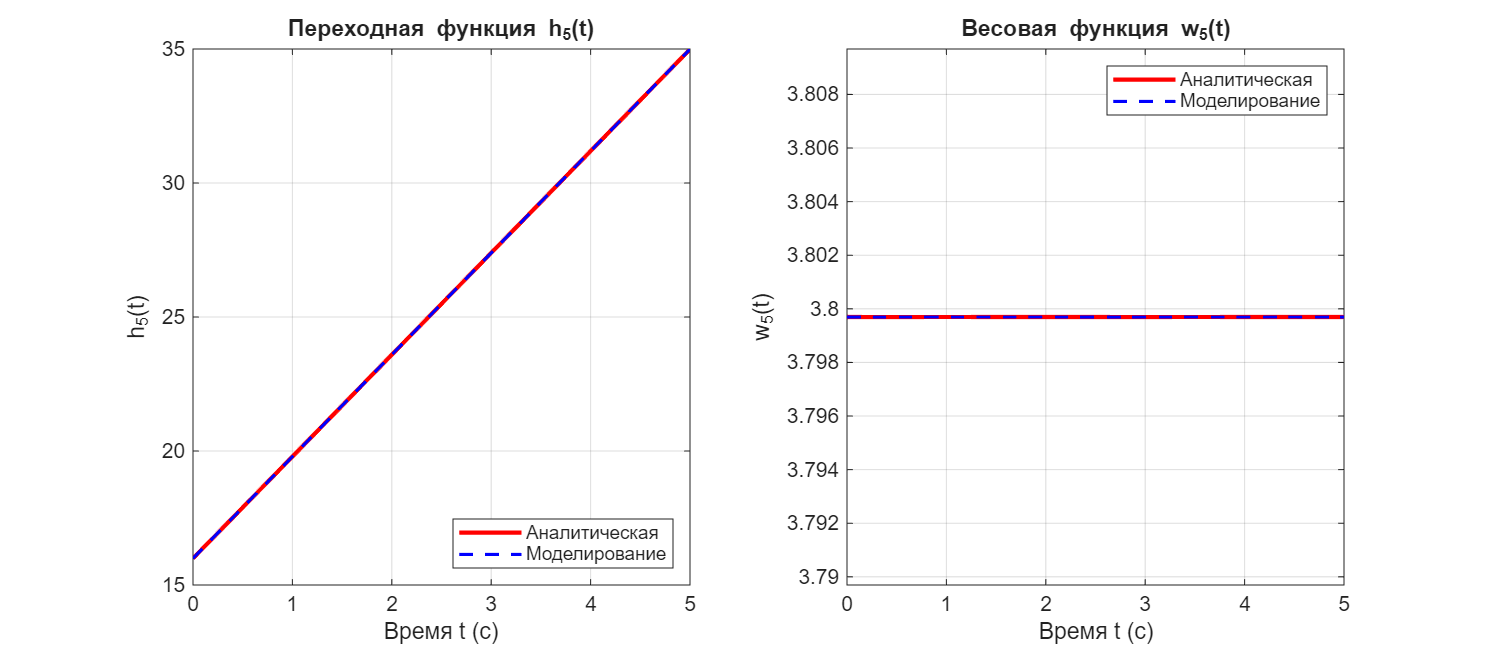
\includegraphics[width=0.85\textwidth]{obj5_time.png}
    \caption{Сравнительные графики переходной $h_5(t)$ и весовой $w_5(t)$ функций Объекта 5}
    \label{fig:obj5_time}
\end{figure}

\begin{figure}[H]
    \centering
    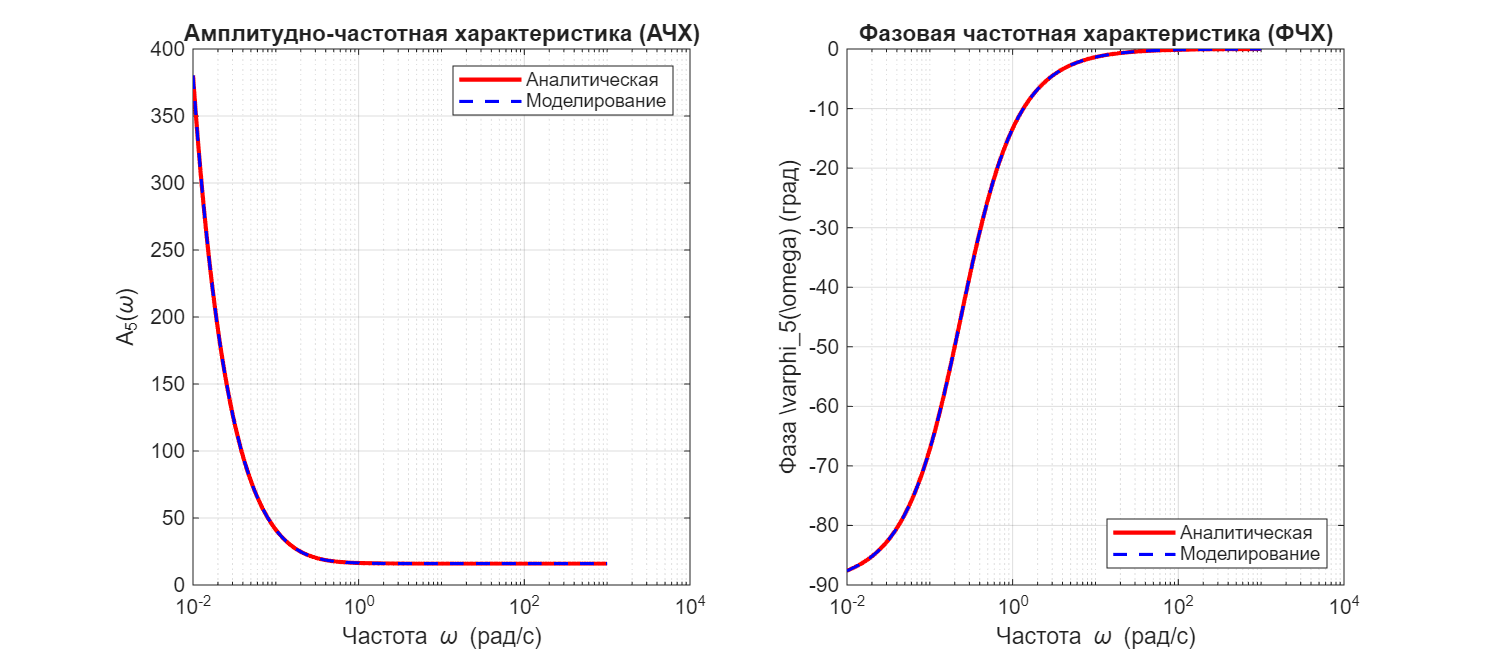
\includegraphics[width=0.85\textwidth]{obj5_freq.png}
    \caption{Сравнительные графики АЧХ и ФЧХ Объекта 5}
    \label{fig:obj5_freq}
\end{figure}

\begin{figure}[H]
    \centering
    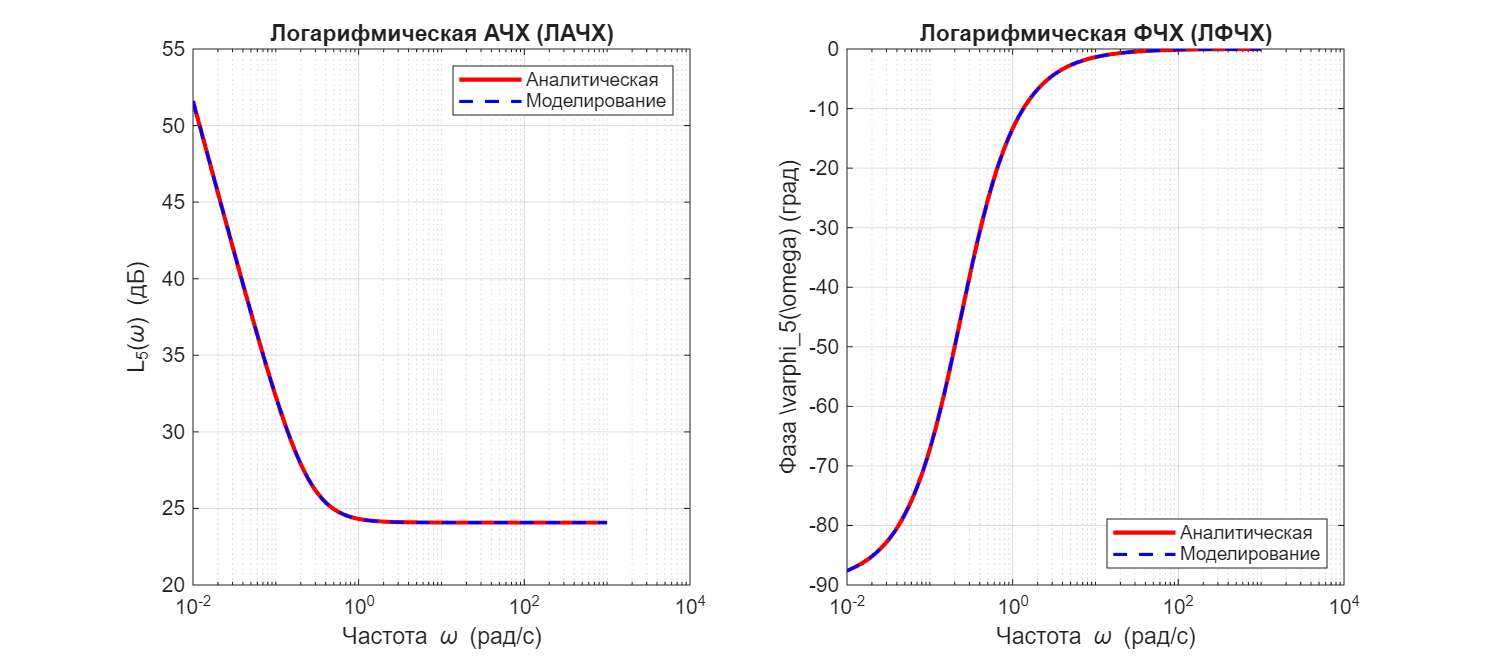
\includegraphics[width=0.85\textwidth]{obj5_bode.png}
    \caption{Сравнительные графики ЛАЧХ и ЛФЧХ Объекта 5}
    \label{fig:obj5_bode}
\end{figure}

По результатам моделирования наблюдается полное совпадение аналитических кривых с результатами компьютерного моделирования в MATLAB:
\begin{itemize}
    \item Переходная характеристика $h_5(t)$ возрастает по линейному закону с начальным скачком, определяемым постоянной времени $T$.
    \item Весовая функция $w_5(t)$ в установившемся режиме стремится к постоянному уровню $K$.
    \item Частотные характеристики отражают свойства корректирующего звена с интегрирующими свойствами на низких частотах.
\end{itemize}

% -----------------------------------------------------------
\subsection{Выводы по Объекту 5}

Для регулятора на операционном усилителе (Вариант 3) получена передаточная функция изодромного интегрирующего звена с параметрами $K \approx 3.7997\text{ с}^{-1}$ và $T \approx 4.2089\text{ с}$. Выведены аналитические зависимости временных и частотных характеристик. Сравнение аналитических кривых с результатами моделирования в MATLAB показало их полное совпадение, что подтверждает правильность теоретического анализа цепи с отрицательной обратной связью.

\newpage
\section{Заключение}

В ходе выполнения лабораторной работы были исследованы пять типичных динамических объектов систем автоматического управления (Вариант 3):
\begin{enumerate}
    \item \textbf{Объект 1 (Двигатель постоянного тока без учета индуктивности):} исследован и описан передаточной функцией апериодического звена 1-го порядка, характеризующегося монотонным переходным процессом.
    \item \textbf{Объект 2 (Двигатель постоянного тока с учетом индуктивности):} представлен в виде колебательного звена 2-го порядка с коэффициентом затухания $\xi = 0.2797$, для которого проявился резонансный пик на частотных характеристиках.
    \item \textbf{Объект 3 (Конденсатор):} описан передаточной функцией идеального интегрирующего звена, обеспечивающего линейный рост выходного напряжения во времени при постоянном входном токе.
    \item \textbf{Объект 4 (Пружинный маятник):} смоделирован как консервативное звено (частный случай колебательного звена при $\xi = 0$), демонстрирующее незатухающие колебания и бесконечный резонанс на частоте $\approx 4.9769\text{ рад/с}$.
    \item \textbf{Объект 5 (Регулятор на операционном усилителе):} исследован как изодромное интегрирующее звено (ПИ-регулятор), сочетающее свойства пропорционального преобразования и интегрирования сигнала.
\end{enumerate}

Для каждого из объектов были успешно выведены математические модели (передаточные функции) в стандартизированном виде, получены аналитические выражения временных ($h(t)$, $w(t)$) и частотных ($A(\omega)$, $\varphi(\omega)$, ЛАЧХ, ЛФЧХ) характеристик. 

Проведенное компьютерное моделирование в среде MATLAB с построением сравнительных графиков показало \textbf{полное совпадение аналитических расчетов с результатами численного эксперимента}. Полученные в ходе работы навыки математического описания, анализа и программной симуляции подтверждают глубокое понимание принципов теории автоматического управления.


\newpage
% -----------------------------------------------------------
\section{Приложение}

Ниже приведен полный листинг скрипта MATLAB для расчета параметров и построения сравнительных характеристик Объекта 1.

\begin{lstlisting}[caption={Скрипт MATLAB для исследования Объекта 1}]
clear; clc; close all;

% 1. Исходные параметры (Вариант 3)
km = 0.3637;
ke = 0.3637;
J  = 0.0023;
R  = 4.6050;

% 2. Расчет стандартизированных параметров K и T
K = 1 / ke;
T = (J * R) / (km * ke);
fprintf('K = %.4f, T = %.4f\n', K, T);

% Передаточная функция
s = tf('s');
W1 = K / (T * s + 1);

% 3. Временные характеристики
t = linspace(0, 0.5, 500);
h_sim = step(W1, t);
w_sim = impulse(W1, t);

h_ana = K * (1 - exp(-t / T));
w_ana = (K / T) * exp(-t / T);

% 4. Частотные характеристики
w = logspace(-1, 3, 500);
[mag, phase] = bode(W1, w);
A_sim = squeeze(mag);
phi_sim = squeeze(phase);
L_sim = 20 * log10(A_sim);

A_ana = K ./ sqrt(1 + (T * w).^2);
phi_ana = -atan(T * w) * (180 / pi);
L_ana = 20 * log10(A_ana);
\end{lstlisting}


Ниже приведен листинг скрипта MATLAB для исследования Объекта 2.

\begin{lstlisting}[caption={Скрипт MATLAB для исследования Объекта 2}]
clear; clc; close all;

% 1. Исходные параметры (Вариант 3)
km = 0.3637;
ke = 0.3637;
J  = 0.0023;
R  = 4.6050;
L  = 1.1784;

% 2. Расчет параметров K, T, xi
K = 1 / ke;
T = sqrt((J * L) / (km * ke));
xi = (J * R) / (2 * T * km * ke);
fprintf('K = %.4f, T = %.4f, xi = %.4f\n', K, T, xi);

% Передаточная функция
s = tf('s');
W2 = K / ((T^2)*s^2 + (2*xi*T)*s + 1);

% 3. Временные характеристики
t = linspace(0, 3, 1000);
h_sim = step(W2, t);
w_sim = impulse(W2, t);

sigma_d = xi / T;
omega_d = sqrt(1 - xi^2) / T;
phi_0 = acos(xi);

h_ana = K * (1 - (exp(-sigma_d * t) / sqrt(1 - xi^2)) .* sin(omega_d * t + phi_0));
w_ana = (K * exp(-sigma_d * t) / (T * sqrt(1 - xi^2))) .* sin(omega_d * t);

% 4. Частотные характеристики
w = logspace(-1, 2, 500);
[mag, phase] = bode(W2, w);
A_sim = squeeze(mag);
phi_sim = squeeze(phase);
L_sim = 20 * log10(A_sim);

A_ana = K ./ sqrt((1 - (T*w).^2).^2 + (2*xi*T*w).^2);
phi_ana = -atan2(2*xi*T*w, 1 - (T*w).^2) * (180 / pi);
L_ana = 20 * log10(A_ana);
\end{lstlisting}



Ниже приведен листинг скрипта MATLAB для исследования Объекта 3.

\begin{lstlisting}[caption={Скрипт MATLAB для исследования Объекта 3}]
clear; clc; close all;

% Đảm bảo thư mục images tồn tại
img_dir = fullfile(pwd, 'images');
if ~exist(img_dir, 'dir')
    mkdir(img_dir);
end

% 1. Исходные параметры (Вариант 3)
C = 287 * 10^(-6); % Ф

% 2. Расчет параметра K
K = 1 / C;
fprintf('K = %.4f\n', K);

% Передаточная функция
s = tf('s');
W3 = K / s;

% 3. Временные характеристики
t = linspace(0, 0.05, 500);
h_sim = step(W3, t);
w_sim = impulse(W3, t);

h_ana = K * t;
w_ana = K * ones(size(t));

% Построение и сохранение графиков временных характеристик
figure('Name', 'Объект 3 - Временные характеристики', 'Position', [100, 100, 950, 420]);
subplot(1, 2, 1);
plot(t, h_ana, 'r-', 'LineWidth', 2); hold on;
plot(t, h_sim, 'b--', 'LineWidth', 1.5);
title('Переходная функция h_3(t)');
xlabel('Время t (с)'); ylabel('h_3(t)');
legend('Аналитическая', 'Моделирование', 'Location', 'Southeast'); grid on;

subplot(1, 2, 2);
plot(t, w_ana, 'r-', 'LineWidth', 2); hold on;
plot(t, w_sim, 'b--', 'LineWidth', 1.5);
title('Весовая функция w_3(t)');
xlabel('Время t (с)'); ylabel('w_3(t)');
legend('Аналитическая', 'Моделирование', 'Location', 'Northeast'); grid on;
saveas(gcf, fullfile(img_dir, 'obj3_time.png'));

% 4. Частотные характеристики
w = logspace(0, 5, 500);
[mag, phase] = bode(W3, w);
A_sim = squeeze(mag);
phi_sim = squeeze(phase);

A_ana = K ./ w;
phi_ana = -90 * ones(size(w));

% Построение и сохранение ЛАЧХ и ЛФЧХ
figure('Name', 'Объект 3 - ЛАЧХ и ЛФЧХ', 'Position', [200, 200, 950, 420]);
subplot(1, 2, 1);
L_ana = 20 * log10(A_ana);
L_sim = 20 * log10(A_sim);
semilogx(w, L_ana, 'r-', 'LineWidth', 2); hold on;
semilogx(w, L_sim, 'b--', 'LineWidth', 1.5);
title('Логарифмическая АЧХ (ЛАЧХ)');
xlabel('Частота \omega (рад/с)'); ylabel('L_3(\omega) (дБ)');
legend('Аналитическая', 'Моделирование', 'Location', 'Southwest'); grid on;

subplot(1, 2, 2);
semilogx(w, phi_ana, 'r-', 'LineWidth', 2); hold on;
semilogx(w, phi_sim, 'b--', 'LineWidth', 1.5);
title('Логарифмическая ФЧХ (ЛФЧХ)');
xlabel('Частота \omega (рад/с)'); ylabel('\varphi_3(\omega) (град)');
legend('Аналитическая', 'Моделирование', 'Location', 'Southwest'); grid on;
saveas(gcf, fullfile(img_dir, 'obj3_bode.png'));
\end{lstlisting}



Ниже приведен листинг скрипта MATLAB для исследования Объекта 4.

\begin{lstlisting}[caption={Скрипт MATLAB для исследования Объекта 4}]
clear; clc; close all;

img_dir = fullfile(pwd, 'images');
if ~exist(img_dir, 'dir')
    mkdir(img_dir);
end

% 1. Исходные параметры (Вариант 3)
M = 13;   % кг
k = 322;  % Н/м

% 2. Расчет параметров K и T
K = 1 / k;
T = sqrt(M / k);
fprintf('K = %.6f, T = %.4f\n', K, T);

% Передаточная функция
s = tf('s');
W4 = K / ((T^2)*s^2 + 1);

% 3. Временные характеристики
t = linspace(0, 5, 1000);
h_sim = step(W4, t);
w_sim = impulse(W4, t);

h_ana = K * (1 - cos(t / T));
w_ana = (K / T) * sin(t / T);

figure('Name', 'Объект 4 - Временные характеристики', 'Position', [100, 100, 950, 420]);
subplot(1, 2, 1);
plot(t, h_ana, 'r-', 'LineWidth', 2); hold on;
plot(t, h_sim, 'b--', 'LineWidth', 1.5);
title('Переходная функция h_4(t)');
xlabel('Время t (с)'); ylabel('h_4(t)');
legend('Аналитическая', 'Моделирование', 'Location', 'Northeast'); grid on;

subplot(1, 2, 2);
plot(t, w_ana, 'r-', 'LineWidth', 2); hold on;
plot(t, w_sim, 'b--', 'LineWidth', 1.5);
title('Весовая функция w_4(t)');
xlabel('Время t (с)'); ylabel('w_4(t)');
legend('Аналитическая', 'Моделирование', 'Location', 'Northeast'); grid on;
saveas(gcf, fullfile(img_dir, 'obj4_time.png'));

% 4. Частотные характеристики (АЧХ и ФЧХ)
w = logspace(-1, 1, 1000);
% Tránh điểm cộng hưởng tuyệt đối tại w = 1/T để không bị chia cho 0 trong plot
w(abs(w - 1/T) < 0.001) = []; 

[mag, phase] = bode(W4, w);
A_sim = squeeze(mag);
phi_sim = squeeze(phase);

A_ana = K ./ abs(1 - (T*w).^2);
phi_ana = zeros(size(w));
phi_ana(w > 1/T) = -180;

figure('Name', 'Объект 4 - Частотные характеристики', 'Position', [150, 150, 950, 420]);
subplot(1, 2, 1);
semilogx(w, A_ana, 'r-', 'LineWidth', 2); hold on;
semilogx(w, A_sim, 'b--', 'LineWidth', 1.5);
title('Амплитудно-частотная характеристика (АЧХ)');
xlabel('Частота \omega (рад/с)'); ylabel('A_4(\omega)');
legend('Аналитическая', 'Моделирование', 'Location', 'Northeast'); grid on;

subplot(1, 2, 2);
semilogx(w, phi_ana, 'r-', 'LineWidth', 2); hold on;
semilogx(w, phi_sim, 'b--', 'LineWidth', 1.5);
title('Фазовая частотная характеристика (ФЧХ)');
xlabel('Частота \omega (рад/с)'); ylabel('Фаза \varphi_4(\omega) (град)');
legend('Аналитическая', 'Моделирование', 'Location', 'Southwest'); grid on;
saveas(gcf, fullfile(img_dir, 'obj4_freq.png'));

% 5. ЛАЧХ и ЛФЧХ
figure('Name', 'Объект 4 - ЛАЧХ и ЛФЧХ', 'Position', [200, 200, 950, 420]);
subplot(1, 2, 1);
L_ana = 20 * log10(A_ana);
L_sim = 20 * log10(A_sim);
semilogx(w, L_ana, 'r-', 'LineWidth', 2); hold on;
semilogx(w, L_sim, 'b--', 'LineWidth', 1.5);
title('Логарифмическая АЧХ (ЛАЧХ)');
xlabel('Частота \omega (рад/с)'); ylabel('L_4(\omega) (дБ)');
legend('Аналитическая', 'Моделирование', 'Location', 'Northeast'); grid on;

subplot(1, 2, 2);
semilogx(w, phi_ana, 'r-', 'LineWidth', 2); hold on;
semilogx(w, phi_sim, 'b--', 'LineWidth', 1.5);
title('Логарифмическая ФЧХ (ЛФЧХ)');
xlabel('Частота \omega (рад/с)'); ylabel('Фаза \varphi_4(\omega) (град)');
legend('Аналитическая', 'Моделирование', 'Location', 'Southwest'); grid on;
saveas(gcf, fullfile(img_dir, 'obj4_bode.png'));
\end{lstlisting}


Ниже приведен листинг скрипта MATLAB для исследования Объекта 5.

\begin{lstlisting}[caption={Скрипт MATLAB для исследования Объекта 5}]
clear; clc; close all;

img_dir = fullfile(pwd, 'images');
if ~exist(img_dir, 'dir')
    mkdir(img_dir);
end

% 1. Исходные параметры (Вариант 3)
R1 = 917;
R2 = 14665;
C  = 287 * 10^(-6);

% 2. Расчет параметров K и T
K = 1 / (R1 * C);
T = R2 * C;
fprintf('K = %.4f, T = %.4f\n', K, T);

% Передаточная функция
s = tf('s');
W5 = K * (T * s + 1) / s;

% 3. Временные характеристики
t = linspace(0, 5, 500);
h_sim = step(W5, t);
w_sim = impulse(W5, t);

h_ana = K * (T + t);
w_ana = K * ones(size(t)); % Исключая дельта-функцию для графического построения

figure('Name', 'Объект 5 - Временные характеристики', 'Position', [100, 100, 950, 420]);
subplot(1, 2, 1);
plot(t, h_ana, 'r-', 'LineWidth', 2); hold on;
plot(t, h_sim, 'b--', 'LineWidth', 1.5);
title('Переходная функция h_5(t)');
xlabel('Время t (с)'); ylabel('h_5(t)');
legend('Аналитическая', 'Моделирование', 'Location', 'Southeast'); grid on;

subplot(1, 2, 2);
plot(t, w_ana, 'r-', 'LineWidth', 2); hold on;
plot(t, w_sim, 'b--', 'LineWidth', 1.5);
title('Весовая функция w_5(t)');
xlabel('Время t (с)'); ylabel('w_5(t)');
legend('Аналитическая', 'Моделирование', 'Location', 'Northeast'); grid on;
saveas(gcf, fullfile(img_dir, 'obj5_time.png'));

% 4. Частотные характеристики
w = logspace(-2, 3, 500);
[mag, phase] = bode(W5, w);
A_sim = squeeze(mag);
phi_sim = squeeze(phase);

A_ana = (K * sqrt(1 + (T*w).^2)) ./ w;
phi_ana = (-90 + atan(T*w) * (180/pi));

figure('Name', 'Объект 5 - Частотные характеристики', 'Position', [150, 150, 950, 420]);
subplot(1, 2, 1);
semilogx(w, A_ana, 'r-', 'LineWidth', 2); hold on;
semilogx(w, A_sim, 'b--', 'LineWidth', 1.5);
title('Амплитудно-частотная характеристика (АЧХ)');
xlabel('Частота \omega (рад/с)'); ylabel('A_5(\omega)');
legend('Аналитическая', 'Моделирование', 'Location', 'Northeast'); grid on;

subplot(1, 2, 2);
semilogx(w, phi_ana, 'r-', 'LineWidth', 2); hold on;
semilogx(w, phi_sim, 'b--', 'LineWidth', 1.5);
title('Фазовая частотная характеристика (ФЧХ)');
xlabel('Частота \omega (рад/с)'); ylabel('Фаза \varphi_5(\omega) (град)');
legend('Аналитическая', 'Моделирование', 'Location', 'Southwest'); grid on;
saveas(gcf, fullfile(img_dir, 'obj5_freq.png'));

% 5. ЛАЧХ и ЛФЧХ
figure('Name', 'Объект 5 - ЛАЧХ и ЛФЧХ', 'Position', [200, 200, 950, 420]);
subplot(1, 2, 1);
L_ana = 20 * log10(A_ana);
L_sim = 20 * log10(A_sim);
semilogx(w, L_ana, 'r-', 'LineWidth', 2); hold on;
semilogx(w, L_sim, 'b--', 'LineWidth', 1.5);
title('Логарифмическая АЧХ (ЛАЧХ)');
xlabel('Частота \omega (рад/с)'); ylabel('L_5(\omega) (дБ)');
legend('Аналитическая', 'Моделирование', 'Location', 'Northeast'); grid on;

subplot(1, 2, 2);
semilogx(w, phi_ana, 'r-', 'LineWidth', 2); hold on;
semilogx(w, phi_sim, 'b--', 'LineWidth', 1.5);
title('Логарифмическая ФЧХ (ЛФЧХ)');
xlabel('Частота \omega (рад/с)'); ylabel('Фаза \varphi_5(\omega) (град)');
legend('Аналитическая', 'Моделирование', 'Location', 'Southwest'); grid on;
saveas(gcf, fullfile(img_dir, 'obj5_bode.png'));
\end{lstlisting}


\end{document}


